\documentclass[12pt]{report}

\usepackage[latin1]{inputenc}
\usepackage[english]{babel}
\usepackage[T1]{fontenc}
\usepackage{ae,aeguill}
\usepackage{graphicx}
\usepackage{float}
\usepackage{ifthen}
\usepackage[figure, algoruled, lined]{algorithm2e}
\usepackage{listings}
\usepackage{makeidx}

\setcounter{secnumdepth}{6}
\setcounter{tocdepth}{6}

%\usepackage{hyperref}
\usepackage[left=3cm,top=3cm,right=3cm]{geometry} 

\renewcommand{\labelitemi}{
\includegraphics[width=6pt]{latex/bullet_robocortex}}

\def \rox {{\bf OPENROX}}
\def \roxdir {{openrox}}

\lstloadlanguages{[ANSI]C}
\lstset{
  basicstyle=\small\ttfamily,
  numberstyle=\tiny,
  breaklines=true,
  language=[ANSI]C
}

%\hypersetup{
%  naturalnames=true,
%  pdftitle={OPENROX},
%  pdfauthor={Ezio MALIS},
%  pdfsubject={User Manual}
%}

{\title{\vspace{-2cm}
\includegraphics[width=0.9\columnwidth]{latex/logo_robocortex}\\~\\
{\bf OPENROX} \\~\\ User's Manual of Version 1.0 \\}}

\author{
%  Ezio Malis 
\\~\\
www.robocortex.com
}
\date{}%\today
\makeindex

\begin{document}
\maketitle
\thispagestyle{empty}
\cleardoublepage

\tableofcontents
\thispagestyle{empty}
%\listoffigures
%\thispagestyle{empty}
\cleardoublepage
\thispagestyle{empty}

\chapter{Introduction}
\label{cha:intro}

\rox{} is a computer vision software written in strict ANSI-C
and optimized for real-time applications. The optimization has been performed with SSE 4.2 for x86 processors and Neon for Arm processors.
No extra dependencies are required to compile the software, just the standard C library. The software provides advanced
algorithms that can be used for applications like vision-guided robot
control and augmented reality. \\

Contrarily to standard computer vision software, \rox{} uses {\bf
direct methods} and {\bf dense information} to solve computer vision
problems. This approach is more robust and accurate than sparse
features-based methods, but generally requires high computation
resources. The use of a new fast optimization technique called {\bf
ESM (Efficient Second-order Approximation Method)} allows to use dense
direct methods in real-time. The ESM technique was proved to have a
higher convergence rate (third-order) than the Newton optimization
technique (second-order) while being more efficient.\\

The present version of the \rox{} is composed of the following modules~:

\begin{description}
  \item[Utils]~: module with basic structures and functions used by all the other modules ;
  \item[Maths]~: module with mathematical structures and methods ;
  \item[Model]~: module with structures and functions to handle target models ;
  \item[Vision]~: module with structures and functions for computer vision ;
  \item[Sensor]~: module with structures and functions for handling sensors ;
  \item[Odometry]~: module with structures and methods for visual odometry computation (sensor localization). The output of the module is the pose of the sensor (translation and rotation in the Cartesian space) relative to a target model ;

\end{description}

\section{Quick guide}
\label{sec:install}

\noindent In the directory \roxdir{}, you will find the following directories:

\begin{itemize}
  \item bin~: The directory containing the dynamic libraries and used to build the executable examples. By default, the license file shall be copied to this directory.
  \item doc~: The directory containing the documentation~;
  \item inc~: The directory containing the headers for the various structures and functions~;
  \item lib~: The directory containing the static libraries~;
  \item lic~: The directory containing the license file~;
  \item res~: Directory needed to save example results~;
  \item seq~: The directory containing the sequence of images (.pgm files) used to test the applications. More test sequences can be downloaded from Robocortex website at www.robocortex.com. Instructions are given in eache example file;
  \item src~: Directory containing several examples for using \rox{}. Examples are provided to test the library and commented in order to
help the user understand how to use and make his own application.;
\end{itemize}

\noindent To compile the examples go to the bin directory:
\begin{lstlisting}
cd bin
\end{lstlisting}
then use cmake-gui (can be downloaded from http://www.cmake.org/) to generate the platform specific projects to compile the examples: 
\begin{lstlisting}
cmake-gui ..
\end{lstlisting}
Make sure that cmake-gui is added to the system PATH. 

\section{License file}
\label{sec:license_file}

A license file shall be obtained to use \rox{} and run the example. By default, the license file shall be copied to the "lic" directory. The user can put the file in a different directory by changing the path in the example files.

%\input{intro/coding.tex}

\newpage
\chapter{Utils Module}
\label{cha:utils}

The utils module provides basic structures and functions used by all the other modules. The utils module contains the following sub-modules:

\begin{description}
  \item[Types]~: Module with common macros and types definitions~;
  \item[Error]~: Module with structures and methods for handling errors~;  
  \item[Timer]~: Module with structures and methods for time measurement~;  
  \item[License]~: Module with structures and methods for file manipulation~;

\end{description}

\section{Types}
\label{sec:types}
The standard ANSI C types are renamed with the prefix ``Rox\_'' in order to ensure portability on different devices. 
If you need further information about the renamed types, please refer to the Programmer Manual.

\section{Error}
\label{sec:error}
Most of the \rox{} functions return an error code that can be displayed in human readable format using the following function:

\begin{lstlisting}
Rox_Void rox_error_display (Rox_Error error);
\end{lstlisting}

Error code is 0 when the function exit successfully.

\section{Timer}
\label{sec:timer}

The Timer module contains functions for time measurements. The module
is useful to measure the computation time when
developing.\\

\subsection{The {\tt Rox\_Timer} object}
\label{sse:timer_object}

A \lstinline$Rox_Timer$ object can be defined using the pointer to a \lstinline$Rox_Timer$:
\begin{lstlisting}
typedef struct Rox_Timer_Struct* Rox_Timer;
\end{lstlisting}

The \lstinline$Rox_Timer$ object can be used both under Linux, Windows or MacOS X without any change.  \\

\subsection{Creating/Deleting a {\tt Rox\_Timer}}
\label{sse:timer_creating}

The following function allows to create/delete a \lstinline$Rox_Timer$ object:
\begin {description}
\item [rox\_timer\_new]~: Create a \lstinline$Rox_Timer$ and allocate memory.
\item [rox\_timer\_del]~: Delete a \lstinline$Rox_Timer$ and free memory.
\end {description}

\subsection{Main functions related to {\tt Rox\_Timer}}
\label{sse:timer_methods}

The following functions shall be used for time measurement:

\begin {description}
\item [rox\_timer\_start]~: Start the timer.
\item [rox\_timer\_stop]~: Stop the timer and return the time elapsed since the initialization.
\end {description}

\noindent Example~:

\begin{lstlisting}
   //Create Rox_Timer 
   Rox_Timer timer = 0

   //Create Rox_Timer 
   rox_timer_new(&timer);

   //Start the timer
   rox_timer_start(timer);

   // Here comes the code for which you make time measurements
   ...

   // Stop the timer
   Rox_Float time_ellapsed = rox_timer_stop(timer);

   // Display time elapsed
   printf("Elapsed Time = \%f ms", time_elapsed \n);

   // Delete the timer
   rox_timer_del(&timer);
\end{lstlisting}

Information about timers is available in the Programmer Manual.

\section{License}
\label{sec:license}

\subsection{License activation using a file}
\label{sse:license_activation_file}
The user can activate the \rox{} license by providing a license file to the following function:

\begin{lstlisting}
Rox_Error rox_license_activate_file (const char *filename);
\end{lstlisting}

\subsection{License activation using a serial number}
\label{sse:license_activation_serial_number}
The user can activate the \rox{} license by providing a serial number to the following function:

\begin{lstlisting}
Rox_Error rox_license_activate_serial_number (const Rox_Uint *serial_number);
\end{lstlisting}

Important remark: this mode is mandatory if the the dynamic libraries of \rox{} are distributed.


\newpage
\chapter{Maths Module}
\label{cha:maths}

The maths module provides mathematical structures and methods such as matrix and vector manipulations. The maths module contains the following sub-modules:

\begin{description}
  \item[Linalg]~: Module with structures and methods for linear algebra~;
    \begin{description}
      \item[Matrix]~: Module with structures and methods for matrix manipulation~;
      \item[Special Matrices]~: Module with structures and methods for special matrices manipulation~;
    \end{description}
  \item[Geometry]~: Module with structures and methods for geometry.
\end{description}

\section{Linear Algebra}
\label{sec:linalg}

The linear algebra module contains method to manipulate vectors, vector spaces, linear maps and systems of linear equations. 

\subsection{Matrix}
\label{sse:matrix}

The matrix module contains matrix definitions and necessary functions to manipulate matrix.

\subsubsection{The {\tt Rox\_Matrix} object}
\label{sss:matrix_object}

A matrix object can be declared using the pointer to a \lstinline$Rox_Matrix_Struct$: 

\begin{lstlisting}
typedef struct Rox_Matrix_Struct* Rox_Matrix;
\end{lstlisting}

The structure is opaque to the user and can only be accessed through constructors, destructors and methods described in the following sections.

\subsubsection{Creating/Deleting a {\tt Rox\_Matrix}}
\label{sss:creating-deleting_matrix}
Functions are provided to allocate, initialize and deallocate an \lstinline$Rox_Matrix$ object~:
\begin{lstlisting}
Rox_Error rox_matrix_new(Rox_Matrix* matrix, const Rox_Uint cols, const Rox_Uint rows);
\end{lstlisting}
The \lstinline$rox_matrix_new$ function allocates memory for data. 
In this case, the size of allocated memory depends of parameters `cols' and `rows'.\\ 

% \begin{lstlisting}
% Rox_Matrix rox_matrix_new_init	(const Rox_Uint cols,
% 				 const Rox_Uint rows,
% 				 const Rox_Real *data);
% \end{lstlisting}
% The \lstinline$rox_matrix_new_init$ function first allocates memory with the default constructor and then copies the parameter `data' to initialize matrix.\\

% \begin{lstlisting}
% Rox_Matrix rox_matrix_new_zeros	(const Rox_Uint cols, 
% 		 		 const Rox_Uint rows);
% \end{lstlisting}
% The \lstinline$rox_matrix_new_zeros$ function first allocates memory with the default constructor and sets to 0 all matrix elements.\\

\begin{lstlisting}
Rox_Error rox_matrix_del(Rox_Matrix * M);
\end{lstlisting}
The \lstinline$rox_matrix_del$ function deallocates memory for an \lstinline$Rox_Matrix$ structure. It is necessary to call this function when the structure is not used any more or before overwriting it.

\subsubsection{Main functions related to {\tt Rox\_Matrix}}
\label{sss:matrix_function}
Several functions are provided for handling matrices. \\

Firstly, it is possible to get / set information from \lstinline$Rox_Matrix$ structure:
\begin{description}
  \item[rox\_matrix\_get\_rows]~: Returns the number of rows of the matrix.
  \item[rox\_matrix\_get\_cols]~: Returns the number of columns of the matrix.
%  \item[rox\_matrix\_get\_size]~: Returns the size of the matrix.
%  \item[rox\_matrix\_get\_data]~: Returns the data of the matrix.
  \item[rox\_matrix\_get\_value]~: Returns a value of the matrix.
  \item[rox\_matrix\_set\_value]~: changes a value of the matrix.
  \item[rox\_matrix\_set\_zero]~: Sets to 0 all matrix elements.
  \item[rox\_matrix\_set\_unit]~: Sets the identity matrix.
\end{description}

%{\bf N.B~:} The functions \lstinline$rox_matrix_set_null$ and \lstinline$rox_matrix_set_unit$ are very similar to 
%\lstinline$rox_matrix_new_null$ and \lstinline$rox_matrix_new_unit$, the main difference is that the 
%\lstinline$Rox_Matrix$ structure shall be already allocated when calling
%\lstinline$rox_matrix_set_null$ or \lstinline$rox_matrix_set_unit$.

%\paragraph{Matrix Calculus}
%\label{par:matricial_calculus}

%Many functions have been developed to use matrices, here the most important functions will be described to make basic matrix calculus.
%\begin{description}
%  \item[rox\_matrix\_add]~: Computes the addition of two matrices.
%  \item[rox\_matrix\_sub]~: Computes the subtraction of two matrices.
%  \item[rox\_matrix\_scm]~: Computes the multiplication of a matrix by a scalar.
%  \item[rox\_matrix\_mulmatmat]~: Computes the multiplication of two matrices.
%  \item[rox\_matrix\_transpose]~: Computes the transpose of a matrix.
%  \item[rox\_matrix\_inv]~: Computes the inverse of the matrix.
%\end{description}

Other functions are provided, further information is available in the programmer manual.


\subsection{Special Linear Group 3$\times$3}
\label{sec:matsl3}
The Special Linear Group SL(3) is defined by the set of 3$\times$3 matrices $\bf{H}$ that verify the following constraint:
\[
\det(\bf{H}) = 1
\] 

\subsubsection{The object {\tt Rox\_MatSL3}}
\label{sss:matsl3_object}
~\\~\\
A \lstinline$Rox_MatSL3$ object can be declared using the pointer to a \lstinline$Rox_MatSL3_Struct$: 

\begin{lstlisting}
typedef struct Rox_MatSL3_Struct* Rox_MatSL3;
\end{lstlisting}

The structure is opaque to the user and can only be accessed through constructors, destructors and methods described in the following sections.

\subsubsection{Creating/Deleting a {\tt Rox\_MatSL3}}
\label{sss:matsl3_delnew}
~\\~\\
Functions are provided to allocate, initialize and deallocate an \lstinline$Rox_MatSL3$ object~:
\begin{lstlisting}
Rox_Error rox_matsl3_new(Rox_MatSL3 * H);
\end{lstlisting}
The \lstinline$rox_matsl3_new$ function allocates memory for data. By default, the matrix is initialized to the identity.\\ 

% \begin{lstlisting}
% Rox_Matrix rox_matsl3_new_init(const Rox_Real data[9]);
% \end{lstlisting}
% The \lstinline$rox_matsl3_new_init$ function first allocates memory with the default constructor and then copies the parameter `data' to initialize matrix.
% The data contains the entries of the matrix row by row.\\

\begin{lstlisting}
Rox_Error rox_matsl3_del(Rox_MatSL3 * H);
\end{lstlisting}
The \lstinline$rox_matsl3_del$ function deallocates memory for an \lstinline$Rox_MatSL3$ structure. It is necessary to call this function when the
structure is not used any more or before overwriting it.

\subsubsection{Main functions related to {\tt Rox\_MatSL3}}
\label{sss:matsl3_methods}
~\\~\\

Firstly, it is possible to get / set information from \lstinline$Rox_MatSL3$ structure:
\begin{description}
  \item[rox\_matsl3\_get\_data]~: Get a copy of the data of the matsl3 matrix.
%  \item[rox\_matsl3\_get\_value]~: Returns a value of the matsl3 matrix.
  \item[rox\_matsl3\_set\_data]~: Set the data of the matsl3 matrix.
  \item[rox\_matsl3\_set\_value]~: changes a value of the matrix.
\end{description}

Several functions are provided to use matrices, here the most important functions will be described to make basic matrix calculus.
\begin{description}
  \item[rox\_matsl3\_mulmatmat]~: Computes the multiplication of two matrices.
  \item[rox\_matsl3\_inv]~: Computes the inverse of the matrix.
  \item[rox\_matsl3\_display]~: Display the matrix.
\end{description}

Other functions are provided, further information is available in the programmer manual.

\subsection{Matrices of the Special Euclidean Group}
\label{sse:matse3}
~\\~\\
The Special Euclidean Group SL(3) is defined by the set of 4$\times$4 matrices ${\bf T}$:
\[
{\bf T} = \left[\begin{array}{cc} {\bf R} & {\bf t} \\ 0 & 1 \end{array} \right]
\]
where ${\bf R} \in SO(3)$ is a rotation matrix that verify the following constraint:
\[
{\bf R}^\top {\bf R} = {\bf I}
\] 
Setting:
\[
{\bf R} = \left[ \begin{array}{ccc} r_{11} & r_{12} & r_{13} \\ r_{21} & r_{22} & r_{23} \\ r_{31} & r_{32} & r_{33} \end{array} \right]
\]
and
\[
{\bf t} = \left[ \begin{array}{c}  t_1 \\ t_2 \\ t_3 \end{array} \right]
\]
The matrix ${\bf T}$ can be written as:
\[
{\bf T} = \left[ \begin{array}{cccc} r_{11} & r_{12} & r_{13} & t_1 \\ r_{21} & r_{22} & r_{23} & t_2 \\ r_{31} & r_{32} & r_{33} & t_3 \\ 0 & 0 & 0 & 1 \end{array} \right]
\]

\subsubsection{The object {\tt Rox\_MatSE3}}
\label{sss:matse3}
~\\~\\
A matse3 object can be declared using the pointer to a \lstinline$Rox_MatSE3_Struct$: 

\begin{lstlisting}
typedef struct Rox_MatSE3_Struct* Rox_MatSE3;
\end{lstlisting}

The structure is opaque to the user and can only be accessed through constructors, destructors and methods described in the following sections.

\subsubsection{Creating/Deleting a {\tt Rox\_MatSE3}}
\label{sss:matse3_delnew}
~\\~\\
Functions are provided to allocate, initialize and deallocate an \lstinline$Rox_MatSE3$ object~:
\begin{lstlisting}
Rox_Error rox_matse3_new(Rox_MatSE3 * T);
\end{lstlisting}
The \lstinline$rox_matse3_new$ function allocates memory for data. By default, the matrix is initialized to the identity.\\ 

% \begin{lstlisting}
% Rox_MatSE3 rox_matse3_new_init(const Rox_Real data[12]);
% \end{lstlisting}
% The \lstinline$rox_matse3_new_init$ function first allocates memory with the default constructor and then copies the parameter `data' to initialize matrix. The data contains the entries of the matrix row by row :

% \[
% data = \left\{ \begin{array}{cccccccccccc} r_{11} & r_{12} & r_{13} & t_1 & r_{21} & r_{22} & r_{23} & t_2 & r_{31} & r_{32} & r_{33} & t_3 \end{array} \right\}
% \]

\begin{lstlisting}
Rox_Error rox_matse3_del(Rox_MatSE3 * T);
\end{lstlisting}
The \lstinline$rox_matse3_del$ function deallocates memory for an \lstinline$Rox_MatSE3$ structure. It is necessary to call this function when the
structure is not used any more or before overwriting it.

\subsubsection{Main functions related to {\tt Rox\_MatSE3}}
\label{sss:matse3_methods}
~\\~\\

Firstly, it is possible to get / set information from \lstinline$Rox_MatSE3$ structure:
\begin{description}
  \item[rox\_matse3\_get\_data\_copy]~: Get a copy of the data of the matse3 matrix.
  \item[rox\_matse3\_get\_value]~: Returns a value of the matse3 matrix.
  \item[rox\_matse3\_set\_data]~: Set the data of the matse3 matrix.
  \item[rox\_matse3\_set\_value]~: changes a value of the matrix.
\end{description}

Several functions are provided to use matrices, here the most important functions will be described to make basic matrix calculus.
\begin{description}
  \item[rox\_matse3\_mulmatmat]~: Computes the multiplication of two matrices.
  \item[rox\_matse3\_inv]~: Computes the inverse of the matrix.
  \item[rox\_matse3\_display]~: Display the matrix.
\end{description}

Other functions are provided, further information is available in the programmer manual.


\section{Geometry}
\label{sec:geometry}

This module contains structures and methods for geometry manipulation. \\

The object \lstinline$Rox_Point2D_Double$ and \lstinline$Rox_Point3D_Double$ are made to contain the coordinates of 2D and 3D points.

\begin{lstlisting}
typedef struct Rox_Point2D_Double_Struct Rox_Point2D_Double;
\end{lstlisting}

\begin{lstlisting}
typedef struct Rox_Point3D_Double_Struct Rox_Point3D_Double;
\end{lstlisting}

The structures are defined as follows:

\begin{lstlisting}
struct Rox_Point2D_Double_Struct
{
   /*! The u-axis coordinate in pixel*/
   Rox_Real u;
   /*! The v-axis coordinate in pixel*/
   Rox_Real v;
};
\end{lstlisting}

\begin{lstlisting}
struct Rox_Point3D_Double_Struct
{
   /*! The x-axis coordinate in meters*/
   Rox_Real X;
   /*! The y-axis coordinate in meters*/
   Rox_Real Y;
   /*! The z-axis coordinate in meters*/
   Rox_Real Z;
};
\end{lstlisting}

More information about the use of geometry objects is available in the Programmer Manual


\newpage
\chapter{Vision Module}
\label{cha:vision}

The vision module contains structures and methods for computer vision and contains the following sub-modules:

\begin{description}
% \item[Overlay]~: Module with structures and methods for image overlaying.
\item[Image]~: Module with structures and methods for manipulating several image format~;
\item[Image Mask]~: Module with structures and methods for image mask manipulation.
\item[Image Display]~: Module with structures and methods for image display.
\item[Identification]~: Module with structures and methods for image identification.

\end{description}

%\input{vision/overlay}
\section{Image}
\label{sec:image}

The image module contains structures and methods for manipulating several image formats. 

\subsection{The object {\tt Rox\_Image}}
\label{sse:image_object}

An image object can be declared using the pointer to a \lstinline$Rox_Image_Struct$ structure. 
\begin{lstlisting}
typedef struct Rox_Image_Struct* Rox_Image;
\end{lstlisting}

\subsection{Creating/Deleting a {\tt Rox\_Image}}
\label{sse:image_newdel}

Functions are provided to allocate and deallocate a \lstinline$Rox_Image$ object~:

\begin{lstlisting}
Rox_Error rox_image_new(Rox_Image * image, Rox_Uint cols, Rox_Uint rows);
\end{lstlisting}

The function allocates memory for data depending parameters  `cols' and `rows' which correspond to image size.\\

An image can be created by directly reading a PGM file from disk using the following function:
\begin{lstlisting}
Rox_Error rox_image_new_readpgm (Rox_Image *image, const char *filename);
\end{lstlisting}
The function first allocate memory for the structure with the rows and
cols parameters matching the image file to load. Then it stores the
image data in the image object.

The following function deallocates memory for a \lstinline$Rox_Image$:
\begin{lstlisting}
Rox_Error rox_image_del(Rox_Image * image);
\end{lstlisting}
 It is necessary to call this function when the object is not used anymore.


\subsection{Main functions related to {\tt Rox\_Image}}
\label{sse:image_functs}

Once the object \lstinline$Rox_Image$ has been allocated, it is possible to get information from \lstinline$Rox_Image$.

\begin{description}
% \item [rox\_image\_get\_data]~: Get the pointer of the first pixel intensity values.
  \item [rox\_image\_get\_rows]~: Get the image rows.
  \item [rox\_image\_get\_cols]~: Get the image columns.
\end{description}

An image can be read from a PGM file if the size is compatible.
Typically, we use a \lstinline$rox_image_new_readpgm$ function to
read the first image of a sequence and allocate correctly the
corresponding structure. Then, assuming that all images of a sequence
have the same dimensions, we can re-use the same structure for the
next images, using the \lstinline$rox_image_readpgm$ function. Thus,
the structure is safely allocated while loading the reference image
and the other images are read previously to perform the tracking.
Currently, the only supported format in the library is raw PGM
(Portable Gray Map) \footnote{{http://netpbm.sourceforge.net/doc/pgm.html}}:
\begin{lstlisting}
Rox_Error rox_image_readpgm (Rox_Image image, const char *filename);
\end{lstlisting}
The function returns an error if the dimensions of the image file do not match the dimesions of the allocated image.

External libraries can be easily used to read images from files. Then,
\rox{} allows to input several image formats. The list of
available image formats is given in the enumeration
\lstinline$Rox_Image_Format_Enum$ (see the Programmer Manual for a
complete list):

\begin{lstlisting}
enum Rox_Image_Format_Enum{
     Rox_Image_Format_Grays,
     Rox_Image_Format_YUV422,
     Rox_Image_Format_Color_RGBA,
     Rox_Image_Format_Color_BGRA,
     Rox_Image_Format_Color_ARGB,
     Rox_Image_Format_Color_BGR,
     Rox_Image_Format_Color_RGB
};
\end{lstlisting}

The image data can be set using the following function:
\begin{lstlisting}
Rox_Error rox_image_set_data (Rox_Image image, Rox_Uchar *data, Rox_Uint bytesPerRow, enum Rox_Image_Format format);
\end{lstlisting}
This function transforms an external image buffer to the rox internal
format and store this information inside the Rox\_Image object.  The
input image format shall be a 3 or 4 channel interleaved image
containing Red, Blue and Green channels.  Only one of these channels
(specified by the channel parameter) will be used while converting to
rox internal format.  User needs to specify the exact format of the
input buffer (e.g. RGB, BGR, RGBA, etc.) as it is impossible to guess
it automatically, as well as how many bytes are used per row in the
input image.

Finally, in order to know if an image suitable for identification and odometry computation, the following functions allows to get a quality score.

The first function is fast but do not provide precise information: 
\begin{lstlisting}
Rox_Error rox_image_get_quality_score (Rox_Real *score, Rox_Image image);
\end{lstlisting}

The second function is slower but provides precise information on the quality of an image:
\begin{lstlisting}
Rox_Error rox_image_get_quality_score_precise (Rox_Real *score, Rox_Image image);
\end{lstlisting}

\section{Image mask}
\label{sec:imask}

\subsection{The object {\tt Rox\_Imask}}
\label{sse:imask_object}

The image structures of {\bf \rox} can be coupled with an image mask structure \lstinline$Rox_Imask_Structure$ that contains a mask. % represented as a byte (unsigned char) tab. 

A mask can be declared using the pointer \lstinline$Rox_Imask$ to a \lstinline$Rox_Imask_Structure$:
 
\begin{lstlisting}
typedef struct Rox_Imask_Struct* Rox_Imask;
\end{lstlisting}

\subsection{Creating/Deleting a {\tt Rox\_Imask}}
\label{sse:creating_imask}
Functions are provided to allocate and deallocate a \lstinline$Rox_Imask$ object~:

\begin{lstlisting}
Rox_Error rox_imask_new(Rox_Imask * imask, Rox_Uint cols, Rox_Uint rows);
\end{lstlisting}
The \lstinline$rox_imask_new$ function allocates memory for a mask object. In this case, the size of allocated memory depends on parameters `cols' and `rows'.\\ 

The \lstinline$rox_imask_del$ function deallocates memory for a mask object. 
\begin{lstlisting}
Rox_Error rox_imask_del(Rox_Imask * M);
\end{lstlisting}
It is necessary to call this function when the structure is not used anymore.

\subsection{Main functions related to {\tt Rox\_Imask}}
\label{sse:imask_methods}

To each pixel of an image corresponds a mask information. If a mask byte is set to 0 (zero), then the corresponding pixel shall be ignored. If a mask byte is set to $\sim$0 (bitwise complement to zero), then the corresponding pixel shall be considered.  By default, an image mask is fully set to  $\sim$0 (bitwise complement to zero). \\

The user can easily define his own mask for a given image. The main
application in the tracking algorithm is to define a non-rectangular
reference region. For example, it is possible to define a circle where
all mask bytes inside this circle are set to  $\sim$0 (bitwise complement to zero) and all
others to 0 (zero). Thus the region to track is not a rectangle but a
circle, even if the image structure represents a rectangular region of
interest.\\

The user can create his own functions to set the image mask as he
wants. The only thing to do is to set to 0 the mask bytes
corresponding to ignored pixels and to  $\sim$0 (bitwise complement to zero) all the others.\\

A function is available to fill a mask object with user defined data~:

\begin{lstlisting}
void rox_imask_set_user(Rox_Imask imask, const Rox_Uchar* data);
\end{lstlisting}

\noindent The `imask' parameter is a \lstinline$Rox_Imask$ structure already allocated with \lstinline$rox_imask_new$. 
The second parameter contains the mask values defined by the user. \\

\noindent The following functions are provided to create basic masks:
\begin{description}
  \item[rox\_imask\_set\_zero]~: Sets the mask values to zero.
  \item[rox\_imask\_set\_one]~: Sets the mask values to one.
  \item[rox\_imask\_set\_ellipse]~: Sets a mask with elliptic shape.
%  \item[rox\_imask\_set\_polygon]~: Sets the image mask inside a polygon .
\end{description}

\noindent Example of mask objects settings~:
\begin{lstlisting}
{
  // Create and allocate Rox_Imask structures
  Rox_Uint size = 64; // The mask will be square
  Rox_Imask Ellipse = rox_imask_new(size, size);
  Rox_Imask User_defined = rox_imask_new(size, size);
  Rox_Imask Polygon = rox_imask_new(size, size);
  Rox_Imask Combination = rox_imask_new(size, size);
 
  // Data for the mask defined by the user
  Rox_Uchar Data[size * size];

  // Initialize Data
  for(int i = 0; i<size; i++)
  {
    for(int j = 0; j<size; j++)
	Data[i+j*size] = ~0;
  }

  for(int i = size/2; i<size; i++)
  {
    for(int j = 0; j<size/2; j++)
	Data[i+j*size] = 0;
  }

  for(int i = 0; i<size/2; i++)
  {
    for(j = size/2; j<size; j++)
	Data[i+j*size] = 0;
  }
   
  //Initialize points for polygon data (In this example, it is a triangle)
  const Rox_Uint points [6] = { 4, 3, 50, 32, 14, 57}; 

  // Set Masks
  rox_imask_set_ellipse(Ellipse);
  rox_imask_set_user(User_defined, Data);
  rox_imask_set_polygon(Polygon, points, 3);
  rox_imask_set_and(Combination, Polygon, User_defined);

  // Save masks
  rox_imask_savepgm("Ellipse.pgm", Ellipse);
  rox_imask_savepgm("User.pgm", User_defined);  
  rox_imask_savepgm("Combination.pgm", Combination);
  rox_imask_savepgm("Polygon.pgm", Polygon);

  // Free Memory
  rox_imask_del(User_defined);
  rox_imask_del(Ellipse);
  rox_imask_del(Polygon);
  rox_imask_del(Combination);
}
\end{lstlisting}

In the figure \ref{fig:mask}, you can see the example results.
In order of appearance, the masks are: Ellipse, User, User-Ellipse combination and Polygon. 
\begin{figure}[htbp] 
\begin{center}
 
\includegraphics[width=0.24\textwidth]{vision/figures/Ellipse}  
 
\includegraphics[width=0.24\textwidth]{vision/figures/User}  
 
\includegraphics[width=0.24\textwidth]{vision/figures/And}
 
\includegraphics[width=0.24\textwidth]{vision/figures/Polygon}  \\ 
 \caption{Examples of setting masks.}
\label{fig:mask}
\end{center}
\end{figure} 

\section{Image Display}
\label{sec:idisp}

The image display module contains structures and methods for displaing results on images and saving on disk. 

\subsection{The object {\tt Rox\_Image\_Display}}
\label{sse:idisp_object}

An image display object can be declared using the pointer to a \lstinline$Rox_Image_Display_Struct$ structure. 
\begin{lstlisting}
typedef struct Rox_Image_Display_Struct* Rox_Image_Display;
\end{lstlisting}

\subsection{Creating/Deleting a {\tt Rox\_Image\_Display}}
\label{sse:idisp_newdel}

Functions are provided to allocate and deallocate a \lstinline$Rox_Image_Display$ object~:

\begin{lstlisting}
Rox_Error rox_image_display_new (Rox_Image_Display *image, Rox_Uint cols, Rox_Uint rows);
\end{lstlisting}

The function allocates memory for data depending parameters  `cols' and `rows' which correspond to image size.\\

\begin{lstlisting}
Rox_Error rox_image_display_del (Rox_Image_Display *image);
\end{lstlisting}

The function deallocates memory for a \lstinline$Rox_Image_Display$ object. It is necessary to call this function when the
structure is not used anymore.

\subsection{Main functions related to {\tt Rox\_Image\_Display}}
\label{sse:idisp_functs}

An image can be read from a PGM or PPM file if the size is compatible using the following functions:

\begin{lstlisting}
Rox_Error rox_image_display_readpgm (Rox_Image_Display image, const char *filename);
\end{lstlisting}

\begin{lstlisting}
Rox_Error rox_image_display_readppm (Rox_Image_Display image, const char *filename);
\end{lstlisting}

After drawing the results, the image can be saved on disk using the following functions:

\begin{lstlisting}
Rox_Error rox_image_display_savepgm (const char *filename, Rox_Image_Display image);
\end{lstlisting}

\begin{lstlisting}
Rox_Error rox_image_display_saveppm (const char *filename, Rox_Image_Display image);
\end{lstlisting}

The results of odometry computation can be drwan using the following functions:
\begin{lstlisting}
Rox_Error rox_image_display_draw_projection_model_single_plane (Rox_Image_Display image, Rox_Matrix calib, Rox_MatSE3 pose, Rox_Model_Single_Plane model, Rox_Uint color);
\end{lstlisting}

\begin{lstlisting}
Rox_Error rox_image_display_draw_projection_model_multi_plane (Rox_Image_Display image, Rox_Matrix calib, Rox_MatSE3 pose, Rox_Model_Multi_Plane model, Rox_Uint color);
\end{lstlisting}

\section{Identification}
\label{sec:ident}

The identification module contains structures and methods for the identification of model images and contains the following sub-modules:

\begin{description}

\item[Photoframe identification]~: Module with structures and methods for texture identification using a photoframe around the model image.
\item[Texture identification]~: Module with structures and methods for texture identification. This module allows the user to define textured model images. The identification at run-time is generally slower than the database identification but can be accelerated using a photoframe around the model image.
\item[Database identification]~: Module with structures and methods for model identification in a database.The database identification module needs the generation of a database from an image model. This offline generation step is time consuming but can be performed once and for all. At runtime, the database identification is faster than the texture identification since many computations have already been done offline.
\end{description}

\subsection{Photoframe identification}
\label{sse:ident_photoframe}

\noindent The photoframe identification module performs the identification of textured model images with a black frame around the texture as shown in Figure~\ref{fig:ident_photoframe}. 

\begin{figure}[H]
\centering
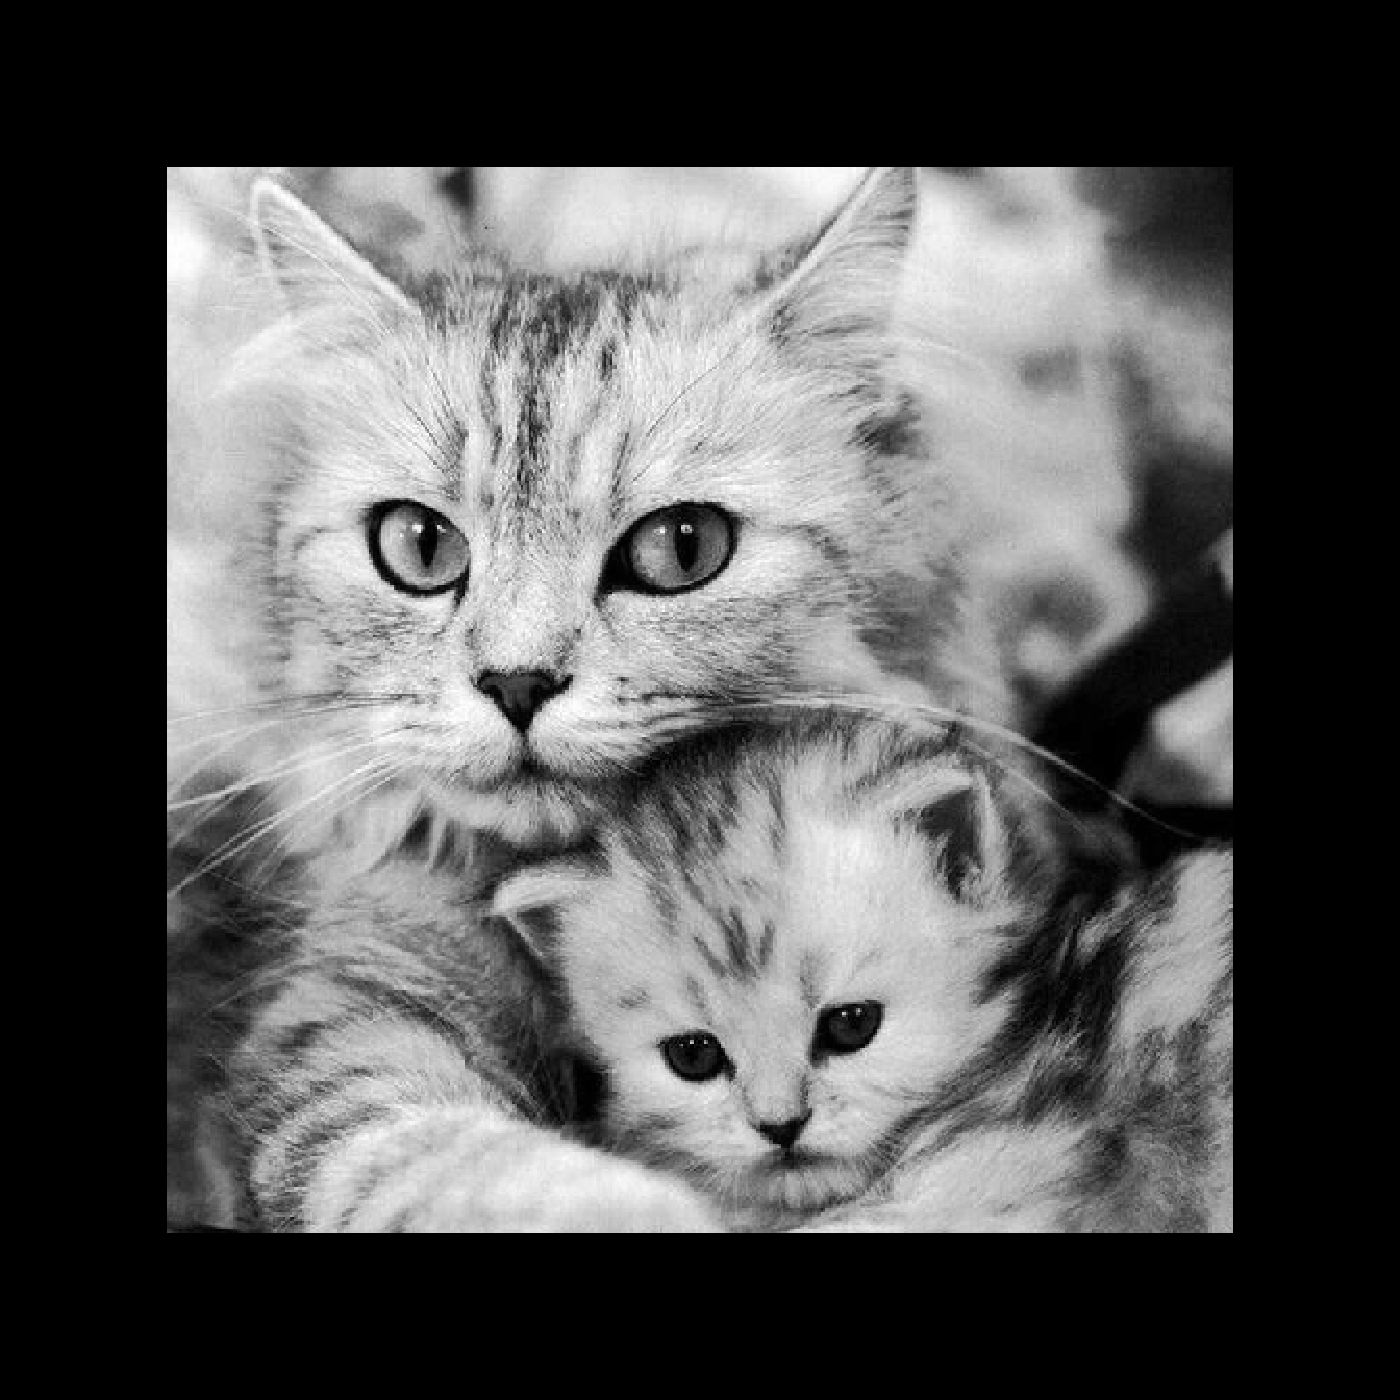
\includegraphics[width=0.45\textwidth]{vision/figures/ident_photoframe} 
\caption{Examples of model that can be identified with the photoframe identification module.}
\label{fig:ident_photoframe}
\end{figure}

The photoframe image model identification is faster than the
identification of phototexture image model since the identification
take benefit of the detection of the black frame around the texture.
On the other hand, the black frame shall be fully visible in the image.

\subsubsection{The {\tt Rox\_Ident\_Photoframe\_SE3} object}
\label{sss:ident_photoframe_object}
A \lstinline$Rox_Ident_Photoframe_SE3$ object is a pointer to the opaque structure \lstinline$Rox_Ident_Photoframe_SE3_Struct$: 

\begin{lstlisting}
typedef struct Rox_Ident_Photoframe_SE3_Struct * Rox_Ident_Photoframe_SE3
\end{lstlisting}

\subsubsection{Creating/Deleting a {\tt Rox\_Ident\_Photoframe\_SE3}}
\label{sss:ident_photoframe_newdel}
~\\

\noindent The rox\_ident\_photoframe object shall be created before any call to other functions using it :

\begin{lstlisting}
Rox_Error rox_ident_photoframe_new(Rox_Ident_Photoframe * ident_photoframe) 
\end{lstlisting}

\noindent This function creates a new empty database object.

\begin{lstlisting}
Rox_Error rox_ident_photoframe_del(Rox_Ident_Photoframe * ident_photoframe)
\end{lstlisting}


\subsubsection{Main functions related to {\tt Rox\_Ident\_Photoframe\_SE3}}
\label{sss:ident_photoframe_functions}
~\\

\noindent A photoframe is a planar object specifically designed to be identified
when filmed with a camera. It is a composition of an image template, a
thick black border and a white background outside of the border.
Figure 1 explains the common scheme of a photoframe.  The image inside
the black borders is the \emph{template}. This template is the object
to identify, and which will be used to track the object after
detection if needed. This template size is
$\left[image \; rows, image \; cols\right]$.  Values iheight and iwidth shall be
equal to 128 pixels.

\begin{figure}[h]
\centering{}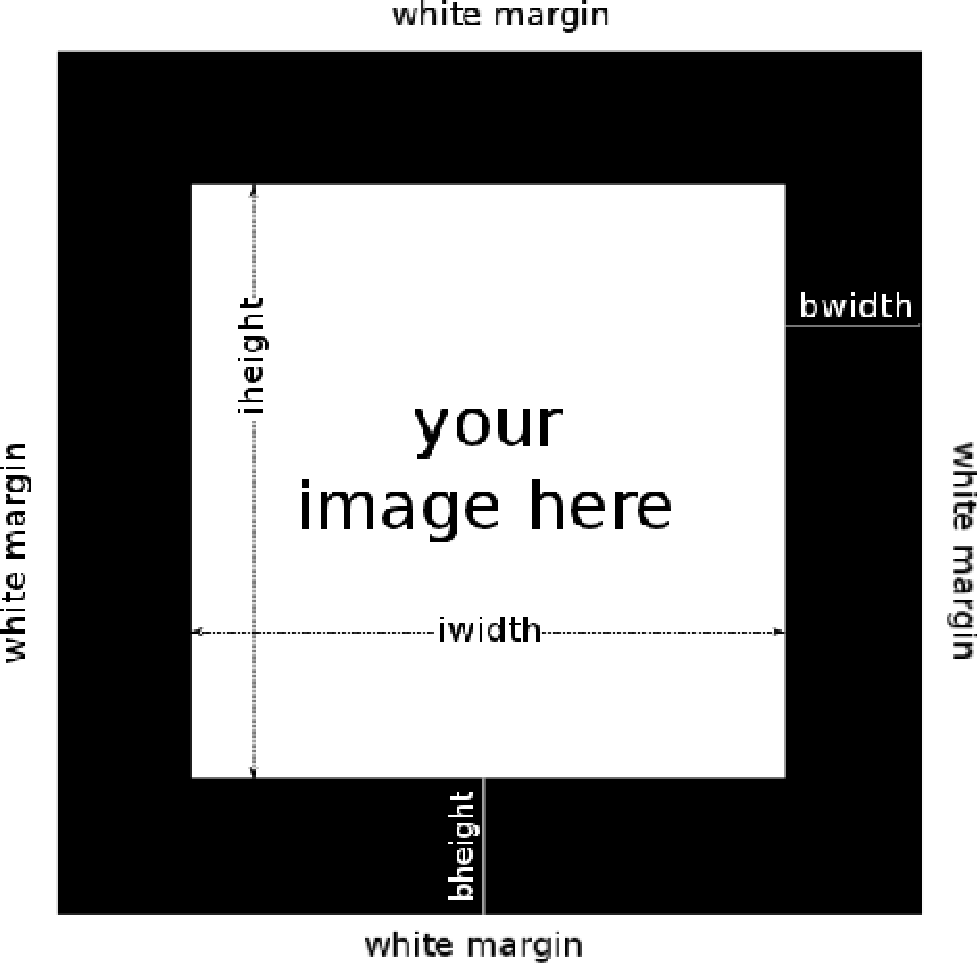
\includegraphics[width=0.6\columnwidth]{vision/figures/fake}
\caption{A common photoframe scheme}
\end{figure}

\noindent The border size $\left[border \; rows, border \;
  cols\right]$ is choosed optimally to be visible in a large set of
viewpoints while not being too large (i.e. not wasting image space).
The following calculus is done to compute border size :

\begin{itemize}
\item border rows = $\frac{80}{512}$ image rows
\item border cols = $\frac{80}{512}$ image cols
\end{itemize}

\noindent Be sure to respect those sizes when creating your photoframe or the
identification performance will be severely degraded.\\

\noindent To create a photoframe, choose a template image which is compatible
with \rox{} (non uniform, with enough texture). Store this template in
a PGM image file. With an image editing software (E.g. : photoshop,
gimp) draw the borders in black color (See figure 1). Print this image
on a white paper sheet. Because of printers approximation, it is not
possible to know what will be the exact size (in meters) of this
print.  Take a ruler to measure the width and height of the image
template \emph{inside} the black borders. These real sizes are only
needed if used to compute odometry after identification. Repeat this
operation for each photoframe you need.\\

\noindent The user can go through the following workflow:

\begin{enumerate}
\item An identification structure is created (see section~\ref{sss:ident_photoframe_newdel}).
\item Template images are added to the identification module using the following function:

\begin{lstlisting}
Rox_Error 	rox_ident_photoframe_se3_addframe (Rox_Ident_PhotoFrame_SE3 obj, Rox_Image model, Rox_Real width_meter, Rox_Real height_meter, Rox_Uint border_width);
\end{lstlisting}

\noindent Adds a new template to a photoframe identification
structure. Shall be called before identification. First parameter is a
pointer created with rox\_ident\_new, second parameter is the template
image to add (without black borders) with a size of 128x128 pixels.
Please note that one photoframe will be identified only once in one
image. If several instances of the same photoframe are in the
processed image, only the first found will be considered. Note that
the identifier of the added photoframe will be the number of times
this function has already been called.

\item The user grabs an image from a stream (e.g. a camera) and gives it
  to photoframe identification. The identification is done and the
  number of identified templates are stored in the \lstinline $Rox_Ident_PhotoFrame_SE3$ object:

\begin{lstlisting}
Rox_Error rox_ident_photoframe_se3_make (Rox_Ident_PhotoFrame_SE3 obj, Rox_Camera camera);
\end{lstlisting}

\noindent Using the ident structure created with rox\_ident\_new and filled
with templates using rox\_ident\_add\_photoframe, tries to detect
photoframes in the given image. This image may be given by a camera
for example. Returns the number of identified photoframes in the current
image.

\item For each template, the user can check if it has been identified using the following function:

\begin{lstlisting}
Rox_Error rox_ident_photoframe_se3_getresult (Rox_Uint *is_identified, Rox_MatSE3 pose, Rox_Ident_PhotoFrame_SE3 obj, Rox_Uint id);
\end{lstlisting}

\noindent Used after a call to rox\_ident\_photoframe. Checks if a given photoframe
(using its id) has been detected or not. ident is a
pointer to a photoframe identification structure created with rox\_ident\_new.
photoframe\_id is a number between 0 and the number of added frames.
Returns Rox\_True if the specific photoframe is detected, Rox\_False
otherwise.

% \item If the template is identified, a function returns a 2D transformation which
% measures how the template is ``seen'' in the current grabbed image.

% \begin{lstlisting}
% Rox_MatSL3 rox_ident_photoframe_get_matsl3(Rox_Ident ident, Rox_Uint id);
% \end{lstlisting}

\noindent Used after a call to rox\_ident\_photoframe and rox\_ident\_get\_identified.
If a photoframe with id has been identified, returns the 2D
transformation which represents the template image (without the borders)
in the current image. 2D transformation is not defined (and may contain
random value) if the marker is not identified.\\

\item Once not used anymore, the identification structure shall
be deleted (see section~\ref{sss:ident_photoframe_newdel}).
\end{enumerate}

\subsection{Texture identification}
\label{sse:ident_texture}

\noindent The texture identification module performs the identification of textured model images as shown in Figure~\ref{fig:ident_texture}. 

\begin{figure}[H]
\centering
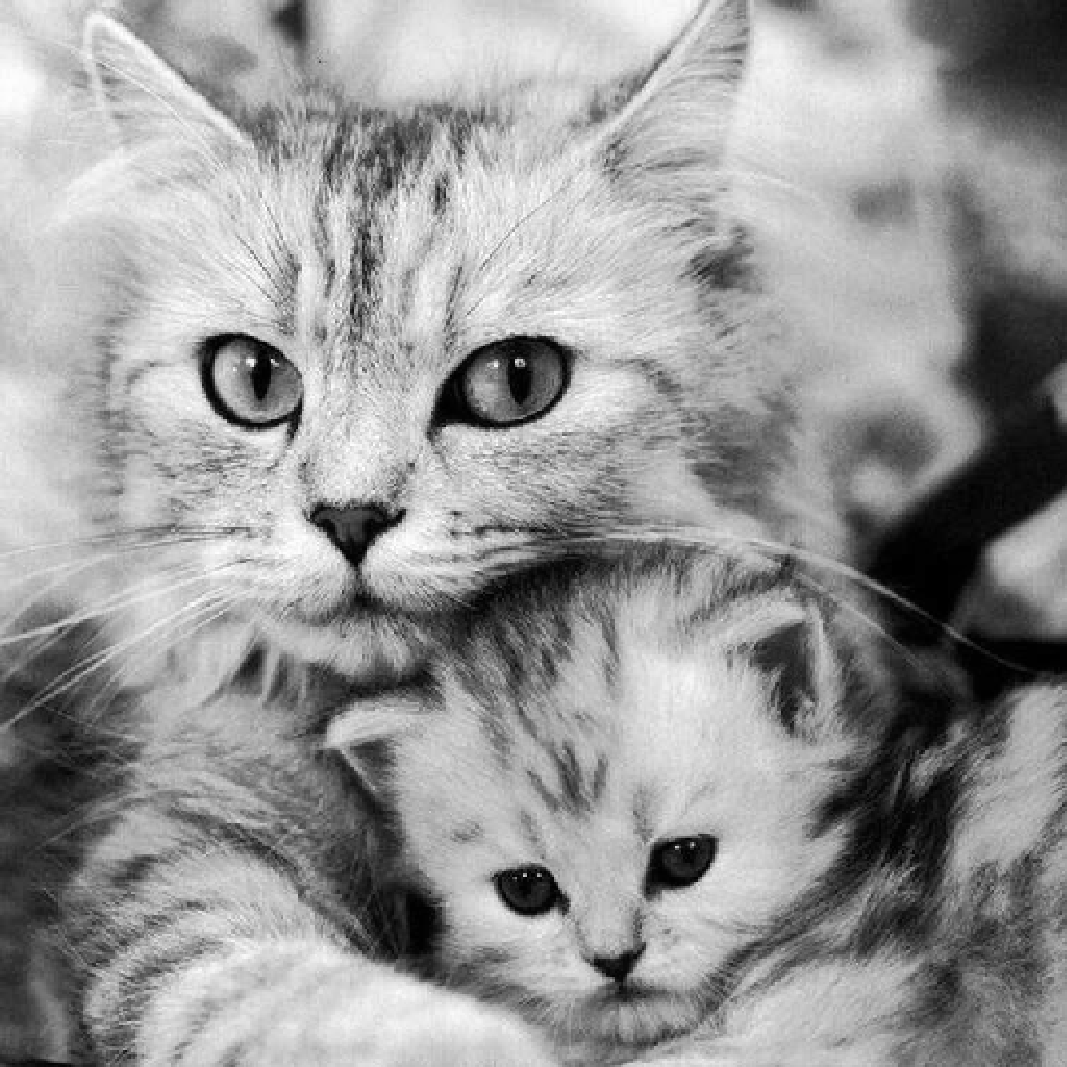
\includegraphics[width=0.45\textwidth]{vision/figures/ident_phototexture} 
\caption{Example of image model that can be identified with the texture identification module.}
\label{fig:ident_texture}
\end{figure}

\subsubsection{The {\tt Rox\_Ident\_Texture\_SE3} object}
\label{sss:ident_texture_object}
A \lstinline$Rox_Ident_Texture_SE3$ object is a pointer to the opaque structure \lstinline$Rox_Ident_Texture_SE3_Struct$: 

\begin{lstlisting}
typedef struct Rox_Ident_Texture_SE3_Struct * Rox_Ident_Texture_SE3
\end{lstlisting}


\subsubsection{Creating/Deleting a {\tt Rox\_Ident\_Texture\_SE3}}
\label{sss:ident_texture_newdel}

\noindent Functions are provided to allocate and deallocate a \lstinline$Rox_Ident_Texture_SE3$ object~:

\begin{lstlisting}
Rox_Error rox_ident_texture_se3_new (Rox_Ident_Texture_SE3 *ident_texture);
\end{lstlisting}

\noindent The function creates a new identification structure. Shall be called before
any other function of this module. Returns a pointer to the Rox\_Ident\_Texture object. \\

\begin{lstlisting}
Rox_Error 	rox_ident_texture_se3_del (Rox_Ident_Texture_SE3 *ident_texture); 
\end{lstlisting}

\noindent Deletes an identification structure. First parameter is a pointer
created with rox\_ident\_texture\_new. Shall be called to free up memory when
user does not need identification anymore.

\subsubsection{Main functions related to {\tt Rox\_Ident\_Texture\_SE3}}
\label{sss:ident_texture_functions}
~\\

A model to be identified can be set using the following function:
\begin{lstlisting}
Rox_Error rox_ident_texture_se3_set_model (Rox_Ident_Texture_SE3 ident_texture, Rox_Model_Single_Plane model); 
\end{lstlisting}
A function is available to identify a given model in a camera object: 
The second function input the camera containing the current image in which to identify the texture:
\begin{lstlisting}
Rox_Error rox_ident_texture_se3_make (Rox_MatSE3 pose, Rox_Ident_Texture_SE3 ident_texture, Rox_Camera camera);
\end{lstlisting}

% If identification is successfull, the resulting homography matrix locating the serched texture in the image can be obtained with the following function: 
% \begin{lstlisting}
% Rox_Bool rox_ident_texture_get_matsl3_copy(Rox_MatSL3 H, Rox_Ident_Texture ident_texture)
% \end{lstlisting}

%\begin{lstlisting}
%Rox_MatSL3 rox_ident_texture_get_matsl3(Rox_Ident_Texture ident_texture) 	
%\end{lstlisting}

\subsection{Database identification}
\label{sse:database}

The computation of visual information (e.g. keypoints features) needed
for image identification can be done offline and stored in a database.
For each image model we would like to identify in the current image, a
specific database item is created. Several items can also mixed
together to allow the identification of multiple images.

Figure~\ref{fig:ident_database} illustrates the structure of the database identification module:

\begin{figure}[H]
\centering
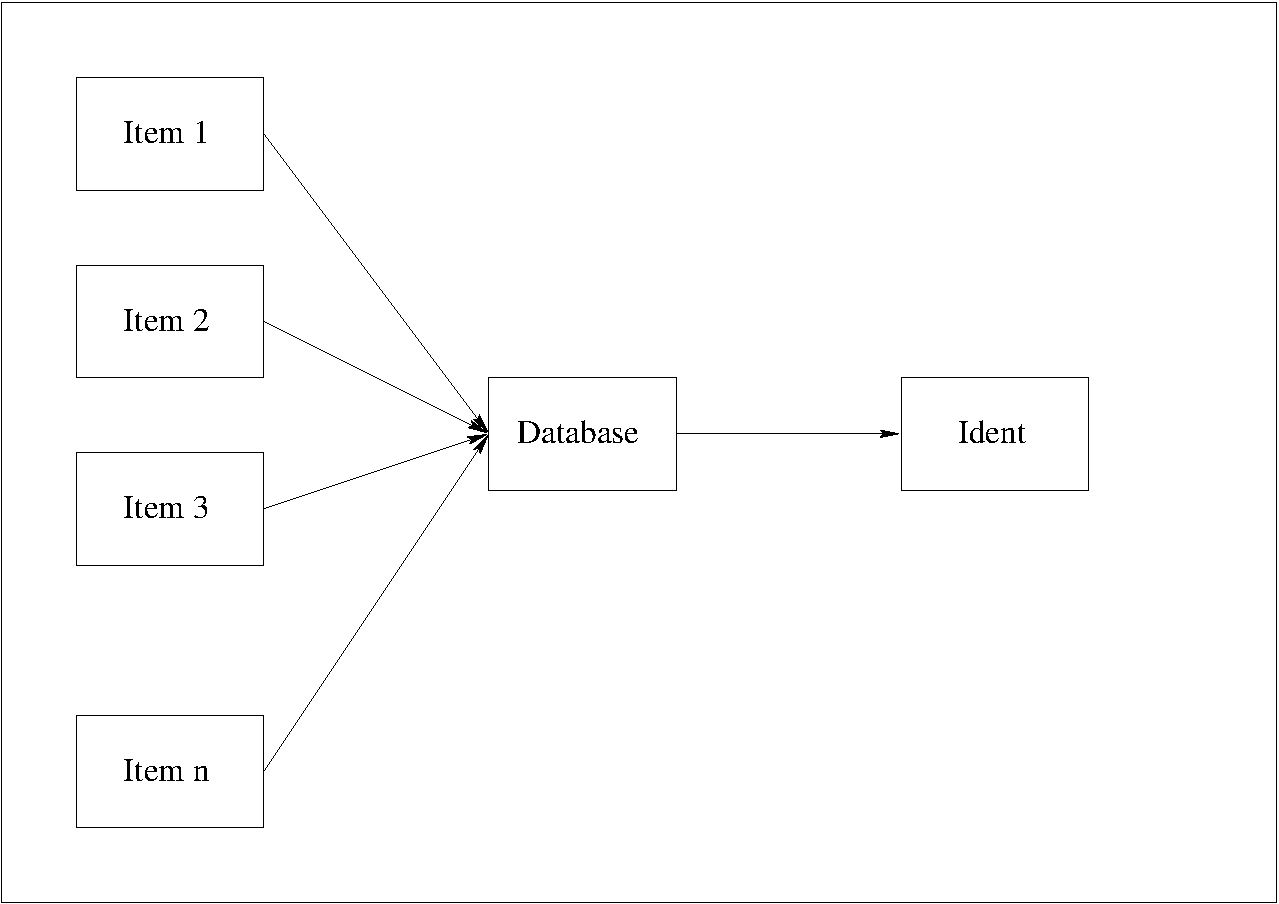
\includegraphics[width=0.75\textwidth]{vision/figures/ident_database} 
\caption{Structure of the database identification module.}
\label{fig:ident_database}
\end{figure}

\subsubsection{The {\tt Rox\_Ident\_Database\_SE3} object}
A \lstinline$Rox_Ident_Database_SE3$ object is a pointer to the opaque structure \lstinline$Rox_Ident_Database_SE3_Struct$: 

\begin{lstlisting}
typedef struct Rox_Ident_Database_SE3_Struct * Rox_Ident_Database_SE3
\end{lstlisting}

\subsubsection{Creating/Deleting a {\tt Rox\_Ident\_Database\_SE3}}

\noindent One database item is associated to one template. A Rox\_Ident\_Database may be considered as a collection of such database items. The database identification module is able to identify several templates simultaneously. Current library is optimized to run on up to 150 simultaneous templates. User can ask the module to detect all possible templates in the same current image or to detect only the most visible template (among the templates in the database). Speed degrades with the number of templates to track simultaneously and quality degrades with the number of templates in the database. It is possible to create several Rox\_Ident\_Database objects in the same program.\\

\noindent The rox\_ident\_database object shall be created before any call to other functions using it :

\begin{lstlisting}
Rox_Error rox_ident_database_se3_new (Rox_Ident_Database_SE3 *ident, Rox_Uint max_templates_simultaneous);
\end{lstlisting}

\noindent This function creates a new empty database object.

\begin{lstlisting}
Rox_Error rox_ident_database_se3_del (Rox_Ident_Database_SE3 *ident);
\end{lstlisting}

This function deletes the object. Shall be called when you do not need this database object anymore.

\subsubsection{Main functions related to {\tt Rox\_Ident\_Database\_SE3}}

% \begin{lstlisting}
% Rox_Bool rox_ident_database_add_template(Rox_Ident_Database
% obj, Rox_Char * pathtodb, Rox_Uint template_height, Rox_Uint template_width)
% \end{lstlisting}

% \noindent This function adds a template database file to the Rox\_Ident\_Database object. Please take care not to add several times the same database file. Template dimensions (template\_height and template\_width) are the dimensions of
% the reduced image to be used for further tracking process. Each time you add a
% template, an internal counter is incremented. The value of this counter is used
% as a unique ID for this template. Thus the template ID is a number between
% 0 and N-1 (N being the number of added templates).

\noindent The following function shall be called to enable
identification and prepare internal structures for optimized
execution:
\begin{lstlisting}
Rox_Error rox_ident_database_se3_set_database (Rox_Ident_Database_SE3 ident, Rox_Database db);
\end{lstlisting}

\noindent The following function execute identification process on the
image contained in the camera object. Uses all the templates added and
compiled before the call to this function. Once a template is found,
an internal flag is set and it will be ignored in further calls to
rox\_ident\_database\_process.
\begin{lstlisting}
Rox_Error rox_ident_database_se3_make (Rox_Ident_Database_SE3 ident, Rox_Camera camera);
\end{lstlisting}

\noindent To get the identification result for a given template ID use the following function: 

\begin{lstlisting}
Rox_Error rox_ident_database_se3_getresult (Rox_Uint *is_identified, Rox_MatSE3 pose, Rox_Ident_Database_SE3 ident, Rox_Uint id); 
\end{lstlisting}

\subsubsection{Creation of database items}

\noindent First, retrieve an image of your template without any perspective distortion. The biggest the image is, the better the detection will perform after database creation. However, if the image is too big the database file will be large and long to create. Ideally, the template size should be close to the image that will be viewed by the camera. The template image shall not contain large textureless regions and shall contain visual information everywhere. Please keep both files in a directory as they will be necessary for identification process.

The programmer can create its own database items by using the following function:
\begin{lstlisting}
Rox_Error rox_database_item_learn_template (Rox_Database_Item item, Rox_Image template); 
\end{lstlisting}

A database item can be saved on disk (use the extension ``.rdi'' for database items) using the following function:
\begin{lstlisting}
Rox_Error rox_database_item_save (Rox_Char *filename, Rox_Database_Item item);
\end{lstlisting}
A database item can be loaded using the following function:
\begin{lstlisting}
Rox_Error rox_database_item_load (Rox_Database_Item item, Rox_Char *filename);
\end{lstlisting}

%The programmer can create its own database item (extension .rdb) by using the following function:
%\begin{lstlisting}
%Rox_Bool rox_ident_database_create(const char *rdb_filename, Rox_Image image)
%\end{lstlisting}

\subsubsection{Creation of a database}

\noindent A database object shall be created using the following function:

\begin{lstlisting}
Rox_Error rox_database_new (Rox_Database *db));
\end{lstlisting}

\noindent This function creates a new empty database object.

The following function deletes the object.

\begin{lstlisting}
Rox_Error rox_database_del (Rox_Database *db); 
\end{lstlisting}
Shall be called when you do not need this database object anymore.

A database item can be added to the database using the following function:

\begin{lstlisting}
Rox_Error rox_database_add_item (Rox_Database database, Rox_Database_Item item, Rox_Real sizx, Rox_Real sizy);
\end{lstlisting}

After adding several items to the database, they can be fused in the database using the following function:

\begin{lstlisting}
Rox_Error rox_database_compile (Rox_Database database);
\end{lstlisting}

The resulting database can be saved on disk (use the extension ``.rdb'' for databases) using the following function:

\begin{lstlisting}
Rox_Error rox_database_save (char *filename, Rox_Database database);
\end{lstlisting}

and loaded from disk using the following function:

\begin{lstlisting}
Rox_Error rox_database_load (Rox_Database db, char *filename);
\end{lstlisting}

For client/server applications the user can serialise a database using the following function:
\begin{lstlisting}
Rox_Error rox_database_serialize (char *buffer, Rox_Database db);
\end{lstlisting}
and after sending it through the network, the user can deserialise it using the following function:
\begin{lstlisting}
Rox_Error rox_database_deserialize (Rox_Database db, char *buffer);
\end{lstlisting}

\subsubsection{Identification using database features directly}

In some applications, like cloud client/server applications, it is useful to store and use directly database features for the identifications. The features are stored in a Rox\_Database\_Features object. 

The programmer can use the following function to create database features:
\begin{lstlisting}
Rox_Error rox_database_features_new (Rox_Database_Features *features);
\end{lstlisting}

The Rox\_Database\_Features object can be deleted using the following function:
\begin{lstlisting}
Rox_Error rox_database_features_del (Rox_Database_Features *features);
\end{lstlisting}

The reference image can be therefore identified using the database features:
\begin{lstlisting}
Rox_Error rox_ident_database_se3_make_features (Rox_Ident_Database_SE3 ident, Rox_Database_Features features, Rox_Matrix calib_camera);
\end{lstlisting}


In the first case, the programmer can also serialize/deserialize the information in the Rox\_Database\_Features object in order to be sent through a network socket: 
\begin{lstlisting}
Rox_Error rox_database_features_serialize (Rox_Char *buffer, Rox_Database_Features features);
\end{lstlisting}

\begin{lstlisting}
Rox_Error rox_database_features_deserialize (Rox_Database_Features features, Rox_Char *buffer);
\end{lstlisting}

In the second case, the file containing the database features can be
created using the following function:
\begin{lstlisting}
Rox_Error rox_database_features_save (Rox_Char *filename, Rox_Database_Features features);
\end{lstlisting}
The file can be loaded using the following function:
\begin{lstlisting}
Rox_Error rox_database_features_load (Rox_Database_Features features, Rox_Char *filename);
\end{lstlisting}

See the example ``rox\_example\_identification\_database\_cloud.c'' for an example of use.

%\subsection{Offline identification}
\label{sse:ident_offline}

\noindent The offline identification module performs the identification of textured model images similarly to the texture identification module. However, higher precision and rate of success are targeted. Thus, the offline identification module is generally much slower than the texture identification module and should be used for offline applications.

\subsubsection{Creating/Deleting a {\tt Rox\_Ident}}
\label{sss:ident_newdel}
~\\

\noindent Functions are provided to allocate and deallocate a \lstinline$Rox_Ident$ object~:

\begin{lstlisting}
Rox_Image rox_ident_new(Rox_Void);
\end{lstlisting}

\noindent The \lstinline$rox_ident_new$ creates a new identification structure. Shall be called before
any other function of this module. Returns a Rox\_Ident pointer. \\

\begin{lstlisting}
Rox_Void rox_ident_del(Rox_Ident ident);
\end{lstlisting}

\noindent Deletes an identification structure. First parameter is a pointer
created with rox\_ident\_new. Shall be called to free up memory when
user does not need identification anymore.

\subsubsection{Main functions related to {\tt Rox\_Ident}}
\label{sss:ident_functions}
~\\

\noindent The following functions can be used for the identification of a planar textured object:

\begin{lstlisting}
Rox_Void rox_ident_set_method(Rox_Ident ident, const Rox_Uint method);
\end{lstlisting}

\noindent Set the identication method:
\begin{itemize}
\item method = 2 : fast identification method but less robust
\item method = 1 : slow identification method but more robust
\item method = 0 : total (try both fast and slow identification methods)
\end{itemize}
The default identification method is 0.

\begin{lstlisting}
Rox_Bool rox_ident_make(Rox_Ident ident, Rox_Image image_model, Rox_Image image_search);
\end{lstlisting}

\noindent Identify the image image\_model into the current image image\_search. Return ROX\_TRUE if the image\_model is identified in the image\_search.

\begin{lstlisting}
Rox_Void rox_ident_get_matsl3_copy(Rox_MatSL3 H, Rox_Ident ident);
\end{lstlisting}

\noindent Get the homographhy matrix H allowing to transform the corners if the model image into the corresponding corners in the image\_search.




\newpage
\chapter{Sensor Module}
\label{cha:sensor}
The sensor module contains structures and methods for sensor manipulation.\\

The sensor module contains the following sub-modules~:

\begin{description}
% \item[Frame]~: Module with structures and methods for frame~;
  \item[Camera ]~: Module with structures and methods for camera sensors~;
%  \item[Camera Calibration]~: Module with structures and methods for camera calibration~;
  \item[Inertia]~: Module with structures and methods for inertia sensing~;
\end{description}


\section{Camera}
\label{sec:camera}
\rox assumes that images are acquired by a camera that respects a standard pin-hole model. 
With this model, straight lines in the 3D space will project to straight lines in the 2D image space.

In a pin-hole model, the relation between a point M with coordinates
(X,Y,Z,1) in reference frame and its equivalent with homogeneous
coordinates (u,v,1) in the camera frame can be written as follows~:
\begin{center}
$
\left( \begin{array}{c} u \\ v \\ 1 \\ \end{array} \right) \propto
\underbrace{\left[ \begin{array}{ccc} f & s & c_u \\ 0 & f r & c_v \\ 0 & 0 & 1 \end{array} \right]}_{\mbox{\footnotesize{K }}} 
\underbrace{\left[ \begin{array}{cccc} & & & t_x \\ & R_{3\times3} & & t_y \\ & & & t_z \\ 0&0&0&1 \end{array} \right]}_{\mbox{\footnotesize{T}}} 
\left( \begin{array}{c} X \\ Y \\ Z \\ 1\\ \end{array} \right)
$
\end{center}

The K matrix corresponds to camera intrinsic parameters where:
\begin{description}
   \item [f]~: Focal lenght in pixels
   \item [r]~: Pixel ratio (equal to 1 for square pixels)
   \item [s]~: Skew (equal to 0 for square or rectangular pixels)
   \item [$c_u$]~: u-coordinate of the optical center projection in the image
   \item [$c_v$]~: v-coordinate of the optical center projection in the image
\end{description}

The intrinsic parameters are generally fixed by the hardware and should not change with time.

The procedure to calibrate the intrinsic parameters is described in the section~\ref{sse:camera_calibration}\\

The T matrix corresponds to camera extrinsic parameters where:
\begin{description}
   \item [R]~: Rotation matrix between reference and current position of the camera
   \item [t]~: Translation vector between reference and current position of the camera
\end{description}

The extrinsic parameters change depending on the camera localization and have to be computed for each image.\\

{\bf \rox} provides functions and structures to handle these parameters. The intrinsic and extrinsic parameters are stored in \lstinline$Rox_Camera$ structure.
% The extrinsic parameters are stored in \lstinline$Rox_Frame$ structure.\\

\subsection{The {\tt Rox\_Camera} object}
\label{sse:camera_struct}

The structure \lstinline$Rox_Camera_Struct$ is designed to hold camera data: intrinsic and extrinsic parameters matrices and the image. 

A camera object is opaque and can be accessed using the pointer \lstinline$Rox_Camera$ to a \lstinline$Rox_Camera_Struct$ structure. 
\begin{lstlisting}
typedef struct Rox_Camera_Struct* Rox_Camera;
\end{lstlisting}

\subsection{Creating/Deleting a {\tt Rox\_Camera}}
\label{sse:camera_newdel}

The library provides functions to create, initialize and delete \lstinline$Rox_Camera$ structure.
\begin{lstlisting}
Rox_Error rox_camera_new (Rox_Camera *camera, Rox_Uint cols, Rox_Uint rows);
\end{lstlisting}
The \lstinline$rox_camera_new$ function allocates memory for data. In this case, the size of allocated memory depends on parameters `cols' and `rows' which correspond to image size. 

% The intrinsic and extrinsic parameters are respectively initialized with `K' and `T'.\\

% If the parameters are unknown, `K' and `T' can be set to NULL.

The \lstinline$rox_camera_new_readpgm$ function allocates memory for data read from a pgm file (`filename'):
\begin{lstlisting}
Rox_Error rox_camera_new_readpgm(Rox_Camera * camera, Rox_Char* filename);
\end{lstlisting}
If the user has a different file format (for example png or jpeg files), he can use its own library to load the image and then fill the Rox\_Image object contained in the Rox\_Camera object (see the Image module).

The \lstinline$rox_camera_del$ function deallocates memory for an \lstinline$Rox_Camera$ structure. It is necessary to call this function when the structure is not used anymore:
\begin{lstlisting}
Rox_Error rox_camera_del(Rox_Camera * camera);
\end{lstlisting}

\subsection{Main functions related to {\tt Rox\_Camera}}
\label{sse:camera_functs}

The main functions to use an \lstinline$Rox_Camera$ structure are~:
\begin{description}
  \item [rox\_camera\_readpgm]~: Sets image field by loading a pgm file.
  \item [rox\_camera\_get\_pose]~: Returns the pointer to the pose matrix.
% \item [rox\_camera\_get\_frame]~: Returns the frame structure.
  \item [rox\_camera\_set\_image]~: Set the image in the camera.
\end{description}
 
\subsection{Camera Calibration}
\label{sse:camera_calibration}

\noindent Camera calibration consists in finding the intrinsic parameters of the following matrix (see section~\ref{sec:camera}):

\begin{equation}
\bf{K} = \left[ \begin{array}{ccc} f & s & c_u \\ 0 & f r & c_v \\ 0 & 0 & 1 \end{array} \right]
\end{equation}

\noindent This tedious procedure is extremely easy with \rox{}.

\noindent The user can print or display on his screen any image with sufficient texture. After measuring the size of the rectangle the user can go through the following work-flow for camera calibration: 

\begin{itemize}
\item create a new calibration object using a 2D model with known size:

\begin{lstlisting}
Rox_Error rox_texture_calibration_mono_perspective_new(Rox_Texture_Calibration_Mono_Perspective *calibration, Rox_Model_2D model);
\end{lstlisting}

The size of the printed texture is given in meters.

\item add a calibration image:
 
\begin{lstlisting}
Rox_Error rox_texture_calibration_mono_perspective_add_image(Rox_Texture_Calibration_Mono_Perspective calibration, Rox_Image image);
\end{lstlisting}

The user shall add images (up to 20) taken with the camera and viewing
the same texture from different point of views. An inclination between
30 and 45 degrees relative to the normal to the texture plane wil
give good results. For optimal results, the texture in the current
image should have almost the ssame size of the model image. The more
images are added, the more camera intrinsic parameters ca be
calibrated (see the ``method'' parameter below).

\item make the camera calibration:
 
\begin{lstlisting}
Rox_Error rox_texture_calibration_mono_perspective_make(Rox_Texture_Calibration_Mono_Perspective calibration, Rox_Uint method);
\end{lstlisting}

The user can choose the ``method'' parameter (between 1 and 5) to calibrate the following camera parameters:

\begin{enumerate}
\item method = 1 : calibrate the focal length $f$ only (assuming the
  principal point $c_u$, $c_v$ are at the center of the image). This
  method needs only 1 image in which the texture model is not observed
  fronto-parallel to the 3D plane.
\item method = 2 : calibrate the focal length $f$ and aspect ration $r$
  (assuming the principal point $c_u$, $c_v$ are at the center of the
  image). This method needs only 1 image in which the texture model is
  not observed fronto-parallel to the 3D plane.
\item method = 3 : calibrate the focal length $f$ and the principal point $c_u$, $c_v$. This method needs at least 2 images in which the texture model is
  not observed fronto-parallel to the 3D plane.
\item method = 4 : calibrate the focal length $f$, aspect ration $r$
  and the principal point $c_u$, $c_v$. This method needs at least 2
  images in which the texture model is not observed fronto-parallel to
  the 3D plane.
\item method = 5 : calibrate the focal length $f$, aspect ration $r$, skew $s$
  and the principal point $c_u$, $c_v$. This method needs at least 3
  images in which the texture model is not observed fronto-parallel to
  the 3D plane.
\end{enumerate}

Use the method number 4 when calibrating the camera for computing the odometry with \rox{}.

\item get the camera calibration:

\begin{lstlisting}
Rox_Error rox_texture_calibration_mono_perspective_get_intrinsics(Rox_Matrix intrinsics, Rox_Texture_Calibration_Mono_Perspective calibration);
\end{lstlisting}

The camera intrinsic parameters are written in a 3x3 matrix.
\end{itemize}

See the example ``rox\_example\_camera\_calibration.c'' for an example of camera calibration.


\section{Inertia}
\label{sec:inertia}

The inertia module, only used for the visual - inertial odometry, is composed by two sub-modules. The {\tt Rox\_Inertial} object contains the accelerometer ($m/s^2$), gyrometer ($rad/s$) and magnetometer calibrated measures and the acquisition timestamp. This data is required by the visual - inertial odometry and available through the {\tt Rox\_Inertial} object. Indeed, after setting the {\tt Rox\_Inertial} object with valid data, the user is able to make visual - inertial odometry using the functions described in section \ref{sss:odometry_visual_inertial_methods} and the {\tt Rox\_Inertial} object.

\subsection{The {\tt Rox\_Inertial} object}
\label{sse:inertial_struct}

A \lstinline$Rox_Inertial$ object can be defined using the pointer to a \lstinline$Rox_Inertial_Structure$:
\begin{lstlisting}
typedef struct Rox_Inertial_Struct* Rox_Inertial;
\end{lstlisting}

\subsection{Creating/Deleting a {\tt Rox\_Inertial}}
\label{sse:inertial_newdel}

Functions are provided to allocate and deallocate a \lstinline$Rox_Inertial$ object~:

\begin{lstlisting}
Rox_Error rox_inertial_new (Rox_Inertial *inertial, const Rox_Float frequency);
\end{lstlisting}
The function allocates memory for the inertial object and returns a pointer on the newly created object.

\begin{lstlisting}
Rox_Error rox_inertial_del (Rox_Inertial *inertial);
\end{lstlisting}
The function deallocates memory for a \lstinline$Rox_Inertial$ object. 
It is necessary to call this function when the object is not used anymore. \\

\subsection{Main functions related to {\tt Rox\_Inertial}}
\label{sse:inertial_functs}

The inertial measures can be set in the \lstinline$Rox_Inertial$ object using the following function~:

\begin{lstlisting}
Rox_Error rox_inertial_set_measure(Rox_Inertial inertial, const Rox_Real* A, const Rox_Real* W, const Rox_Real* M, Rox_Real timestamp);
\end{lstlisting}

This function set the accelerometer, gyrometer and magnetometer measures from \lstinline$Rox_Real$ buffers and sets the acquisition timestamp~;

If you need further information about inertial functions, please refer to the Programmer Manual.



\newpage
\chapter{Model Module}
\label{cha:model}
The model module contains structures and methods for model manipulation.\\

The model module contains the following sub-modules~:

\begin{description}
  \item[Model Single Plane]~: Module with structures and methods for single plane models definition and use~;
  \item[Model Multi Plane]~: Module with structures and methods for multi plane models definition and use~;
\end{description}

\section{Model Single Plane}
\label{sec:model_single_plane}

\subsection{The {\tt Rox\_Model\_Single\_Plane} object}
\label{sse:model_single_plane_typedef}
A \lstinline$Rox_Model_Single_Plane$ object can be declared using the pointer to a \lstinline$Rox_Model_Single_Plane_Struct$: 

\begin{lstlisting}
typedef struct Rox_Model_Single_Plane_Struct* Rox_Model_Single_Plane;
\end{lstlisting}

The structure is opaque to the user and can only be accessed through constructors, destructors and methods described in the following sections.

\subsection{Creating/Deleting a {\tt Rox\_Model\_Single\_Plane}}
\label{sse:model_single_plane_newdel}

Functions are provided to allocate, initialize and deallocate an \lstinline$Rox_Model_Single_Plane$ object~:
\begin{lstlisting}
Rox_Error rox_model_single_plane_new(Rox_Model_Single_Plane * model_single_plane, Rox_Image image, Rox_Real sizex, Rox_Real sizey);
\end{lstlisting}
The \lstinline$rox_model_single_plane_new$ function allocates memory for data. \\ 

\begin{lstlisting}
Rox_Error rox_model_single_plane_del(Rox_Model_Single_Plane * model_single_plane);
\end{lstlisting}
The \lstinline$rox_model_single_plane_del$ function deallocates memory for an \lstinline$Rox_Model_Single_Plane$ structure. It is necessary to call this function when the
structure is not used any more or before overwriting it.

\subsection{Main functions related to {\tt Rox\_Model\_Single\_Plane}}
\label{sse:model_single_plane_functs}
The texture (i.e. an image) associated to the planar model can be set using the following function:
\begin{lstlisting}
Rox_Error rox_model_single_plane_set_template(Rox_Model_Single_Plane model, Rox_Image image, Rox_Real sizex, Rox_Real sizey); 
\end{lstlisting}
The real size of the planar target must be given.

\section{Model Multi Plane}
\label{sec:model_multi_plane}
The present version of \rox{} allows the user to define simple 3D objects only.
Currently, the 3D object is described as a set of 3D quadrilaterals (e.g. : the 6 
faces of a cube or parts of the faces). Each quadrilateral is defined by an image 
texture and four 3D points associated to each corner of the texture (order : Top left -> Top
right -> Bottom right -> Bottom left). The 3D vertices of all faces shall be defined 
in a common reference frame $\mathcal{F}_{r}$. Be sure to define your 3D coordinates 
as precisely as possible. It is up to the user to choose the adequate $\mathcal{F}_{r}$ for your vertices.
The default pose estimated by the odometry is the 3D transformation 
(rotation and translation) from this reference frame to the camera frame. 

\subsection{The {\tt Rox\_Model\_Multi\_Plane} object}
\label{sse:model_multi_plane_struct}
A model 3D object is a pointer to the opaque structure \lstinline$Rox_Model_Multi\_Plane_Struct$: 

\begin{lstlisting}
typedef struct Rox_Model_Multi\_Plane_Struct* Rox_Model_Multi\_Plane;
\end{lstlisting}

The structure is opaque to the user and can only be accessed through constructors, destructors and methods described in the following sections.

\subsection{Creating/Deleting a {\tt Rox\_Model\_Multi\_Plane}}
\label{sse:model_multi_plane_newdel}

Functions are provided to allocate, initialize and deallocate an \lstinline$Rox_Model_Multi\_Plane$ object~:
\begin{lstlisting}
Rox_Error rox_model_multi_plane_new(Rox_Model_Multi\_Plane * model_multi_plane);
\end{lstlisting}
The \lstinline$rox_model_multi_plane_new$ function allocates memory for data. \\ 

\begin{lstlisting}
Rox_Error rox_model_multi_plane_del(Rox_Model_Multi\_Plane * model_multi_plane);
\end{lstlisting}
The \lstinline$rox_model_multi_plane_del$ function deallocates memory for an \lstinline$Rox_Model_Multi_Plane$ structure. It is necessary to call this function when the
structure is not used any more or before overwriting it.

\subsection{Main functions related to {\tt Rox\_Model\_Multi\_Plane}}
\label{sse:model_multi_plane_functs}

The main function related to the \lstinline$Rox_Model_Multi_Plane$ is the function that allows to define an additional textured quadrilateral belonging to the 3D object:
\begin{lstlisting}
Rox_Error rox_model_multi_plane_append_plane(Rox_Model_Multi_Plane model, Rox_Image image, Rox_Real vertices[4])
\end{lstlisting}


\newpage
\chapter{Motion Detection Module}
\label{cha:motion_detection}

Visual motion detection is the process of determining the changes
occurring in a sequence of images relative to a given reference
image. If the camera is static, these changes are mainly due to moving
objects. The localization of moving objects in the image is used in
several applications such as robotics, active video-surveillance, and many
others.

In \rox{}, the detection of a moving target is done inside an
appropriate Region Of Interest (ROI) selected by the user. In the
current version of \rox{} the image is supposed to be acquired by a
static camera.

The Detection module contains the following sub-modules:

\begin{description}
\item[Detection Parameters]~: module with structures and methods for handling the detection parameters~;
\item[Detection]~: module with structures and methods for motion detection ~;
\end{description}

\section{Detection Parameters}
\label{sec:detection_params}

\subsection{The Rox\_Detection\_Params object}
\label{sse:detection_params_object}

The object \lstinline$Rox_Detection_Params$ contains two
parameters that can be used to define the visual detection.
 The parameters are the following:

\begin{itemize}
\item Bandwidth : the approximate size of the object to be detected 
\item Sensitivity : the motion detection sensitivity
\end{itemize}

The detection parameters are stored in a \lstinline$Rox_Detection_Params_Struct$ structure. A \lstinline$Rox_Detection_Params$ object is opaque and can be accessed using the pointer to a \lstinline$Rox_Detection_Params_Struct$ structure: 
\begin{lstlisting}
typedef struct Rox_Detection_Params_Struct* Rox_Detection_Params;
\end{lstlisting}

\subsection{Creating/Deleting a Rox\_Detection\_Params object}
\label{sse:detection_params_creating}

\rox{} provides functions to create / delete the Rox\_Detection\_Params structure~:

\begin{lstlisting}
Rox_Detection_Params rox_detection_params_new(Rox_Void);
\end{lstlisting}
The \lstinline$rox_detection_params_new$ function allocates memory for the structure, 
sets parameters with default values (\lstinline$bandwidth = (20x30) pixels$, \lstinline$sensitivity = 1.0$) and returns a pointer on the newly created structure.\\

\begin{lstlisting}
Rox_Void rox_detection_params_del(Rox_Detection_Params Params);
\end{lstlisting}
The \lstinline$rox_detection_params_del$ function deallocates memory for a parameter structure. It
is necessary to call this function when the structure is not used anymore or before overwriting it.

\subsection{Main functions related to the object Rox\_Detection\_Params}
\label{sse:detection_params_functions}

The motion detection algorithm has two important parameters set at the parameters structure
initialization~: `bandwidth', `sensitivity'. Functions are provided to set these parameters~:

\begin{itemize}
  \item \lstinline$rox_detection_params_set_bandwidth$~: Sets the bandwidth parameter which is the approximate size of the moving object to detect. If the bandwidth is small, parts of bigger objects will be detected separately. On the contrary, if the   bandwidth is big, smaller objects may be grouped together. 
  \item \lstinline$rox_detection_params_set_sensitivity$~: Sets sensitivity parameter. The higher the sensitivity the more objects will be detected but false detections may appear (due to lighting changes, noise, or other minor changes in the image).
\end{itemize}

Setting a parameter with a non valid value (for example -1) will leave it unchanged. \\

Finally, the function \lstinline$rox_detection_params_set_license_path$ allows the user to set the path of the license file.


\section{Detection}
\label{sec:detetion}

\subsection{The Rox\_Detection object}
\label{sse:detection_object}

A \lstinline$Rox_Detection$ object can be defined using the pointer to a \lstinline$Rox_Detection_Structure$:
\begin{lstlisting}
typedef struct Rox_Detection_Struct* Rox_Detection;
\end{lstlisting}

\subsection{Creating/Deleting a Rox\_Detection object}
\label{sss:detection_initializing}

Functions are provided to allocate and deallocate a \lstinline$Rox_Detection$ structure~:
\begin{lstlisting}
Rox_Detection rox_detection_new(Rox_Detection_Params detection_params, Rox_Image image);
\end{lstlisting}
The \lstinline$rox_detection_new$ function allocates memory for the structure of the motion detection, according to
the \lstinline$detection_params$ object and returns a pointer on the newly created structure. The input image corresponds to the model image (background) used for the motion detection. \\

\begin{lstlisting}
Rox_Void rox_detection_del(Rox_Detection detection);
\end{lstlisting}
The \lstinline$rox_detection_del$ function deallocates memory for a \lstinline$Rox_Detection$ structure. 
It is necessary to call this function when the structure is not used anymore or before overwriting it. 
Remember to set \lstinline$detection = NULL;$ after deleting the object.
\\

The \lstinline$Rox_Detection$ structure is opaque, i.e. its internal
fields are hidden and cannot be accessed directly by the user. A
consequence is that the user can only declare and manipulate pointer
on this structure, and never the structure itself, as the size of the
structure is unknown to the user.\\

In order to detect moving objects in several ROI, the user can declare and create
several \lstinline$Rox_Detection$ structures and perform the algorithm on each of
them. \\

\subsection{The main functions related to the object Rox\_Detection}
\label{sss:detection_methods}

Once the \lstinline$Rox_Detection$ is allocated and initialized, it is possible to:
\begin{itemize}
  \item Set a different model image
  \item Set an image mask to avoid detection in specific parts of the ROI
  \item Set different parameters for each detection
  \item Detect moving objects
\end{itemize}

\subsubsection{Setting a model image}
\label{sse:detection_set_model}

The function \lstinline$rox_detection_motion_set_model$ allows the
user to set a model image which may be different from the model image
chosen at initialization. This can be useful if the appearance of the
model has changed. For example the detection may start in the morning
and in the afternoon the lighting conditions have changed so much
that it is preferable to renew the model image.\\

\subsubsection{Setting an image mask}
\label{sse:detection_set_imask}

The following functions allow the user to set an image mask of any shape. This mask can be used to avoid
detection in specific parts of the ROI. \\

\paragraph{Setting an image mask from windows}
\label{sss:detection_set_imask_windows}
~\\
The function \lstinline$rox_detection_set_imask_window$ shall be used
to select a rectangular region defined by a window.

The function \lstinline$rox_detection_motion_set_imask_window_list$ shall be used to select several rectangular regions defined by a window list.

\paragraph{Setting an user defined image mask}
\label{sss:detection_set_imask_user}
~\\

The function \lstinline$rox_detection_set_imask$ shall be used for defining such regions (for example a disc).\\
Further information about image masks can be found in section \ref{sec:imask}. Detection can then be performed with
\lstinline$rox_detection_make$ function.

\subsubsection{Setting detection parameters}
\label{sse:detection_set_params}

The motion detection parameters (see section \ref{sec:detection_params}) can be modified for each image using the following functions:

\lstinline$rox_detection_motion_set_bandwidth$

\lstinline$rox_detection_motion_set_sensitivity$

%\paragraph{Setting the size of the detected objetcs}
%\label{sss:detection_set_bandwidth}

%\paragraph{Setting the detection sensitivity}
%\label{sss:detection_set_sensitivity}

\subsubsection{Performing motion detection}
\label{sss:detection_set_params}

To perform the detection we call the \lstinline$rox_detection_make$
function with the \lstinline$Rox_Detection$ structure and the image
used to perform the detection as parameters. This function shall be
called for each image of the sequence in which the user would like to
detect a moving object.

The output of the detection is a list of windows defining a bounding
box around the moving object.

See the example ``rox\_example\_detection.tex'' for an example of use.

%\input{detection/rox_example_detection}

\newpage
\chapter{Tracking Module}
\label{cha:track}

Visual tracking is the process of determining the position of a target
in a sequence of images. The localization of the target in the image
can be useful in several applications such as robotics,
video-surveillance, and many others.

In \rox{}, the selection of the target can be done by the user manually
with a selection of an appropriate Region Of Interest (ROI) in the
reference image. If the user has already defined such an ROI, \rox{} allows to identify a given image model in the current image. The
identification module is also used to re-identify the target if the tracking is
lost (for example if the ROI is occluded or out of the image).

The Tracking module contains the following sub-modules:

\begin{description}
  \item[Tracking Parameters]~: module with structures and methods for handling the tracking parameters~;

  \item[Tracking]~: module with structures and methods for tracking 2D objects~;

\end{description}

\section{Tracking Parameters}
\label{sec:tracking_params}

\subsection{The Rox\_Tracking\_Params object}
\label{sse:tracking_params_object}

The object \lstinline$Rox_Tracking_Params$ contains several
parameters that can be used to define the visual tracking.
The basic shape for an area of interest is a rectangle. However,
the user can also define a region of interest inside a polygon or create
a customized area with image masks. The most important parameters are the following:

\begin{itemize}
\item Iteration number
\item Tracking precision
\item Prediction area
\item Use of Kalman filter
\item Score threshold  
\end{itemize}

The tracking parameters are stored in a \lstinline$Rox_Tracking_Params_Struct$ structure. A \lstinline$Rox_Tracking_Params$ object is opaque and can be accessed using the pointer to a \lstinline$Rox_Tracking_Params_Struct$ structure: 
\begin{lstlisting}
typedef struct Rox_Tracking_Params_Struct* Rox_Tracking_Params;
\end{lstlisting}

\subsection{Creating/Deleting a Rox\_Tracking\_Params object}
\label{sse:tracking_params_creating}

\rox{} provides functions to create / delete the Rox\_Tracking\_Params structure~:

\begin{lstlisting}
Rox_Tracking_Params rox_tracking_params_new(Rox_Void);
\end{lstlisting}
The \lstinline$rox_tracking_params_new$ function allocates memory for the structure, 
sets parameters with default values (\lstinline$miter = 10$, \lstinline$mprec =  0$, \lstinline$mpred = 16$, \lstinline$score_thresh = 0.89$, \lstinline$kalman = ROX_TRUE$, \lstinline$auto_update = ROX_FALSE$, \lstinline$light = ROX_FALSE$) and returns a pointer on the newly created structure.\\

\begin{lstlisting}
Rox_Tracking_Params rox_tracking_params_new_readfile (Rox_File filename);
\end{lstlisting}
The \lstinline$rox_tracking_params_new_readfile$ function allocates memory for the structure,
reads the `filename' \lstinline$Rox_File$ and sets parameters with read values. A pointer on the newly created patch is returned by this function.\\

\begin{lstlisting}
Rox_Void rox_tracking_params_del(Rox_Tracking_Params Params);
\end{lstlisting}
The \lstinline$rox_tracking_params_del$ function deallocates memory for a parameter structure. It
is necessary to call this function when the structure is not used anymore or before overwriting it.

\subsection{The main functions related to the object Rox\_Tracking\_Params}
\label{sse:tracking_params_functions}

The tracking algorithm has four important parameters set at the parameters structure
initialization~: `miter', `mprec', `mpred', `mtime'. Functions are provided to set these parameters~:

\begin{itemize}
%  \item \lstinline$rox_tracking_params_set_mtime$~: Sets mtime parameter~;
  \item \lstinline$rox_tracking_params_set_miter$~: Sets miter parameter~;
  \item \lstinline$rox_tracking_params_set_mprec$~: Sets mprec parameter~;
  \item \lstinline$rox_tracking_params_set_mpred$~: Sets mpred parameter~;
\end{itemize}

Setting a parameter with a strictly negative value (typically -1) will
leave it unchanged. \\

%{\bf Warning :} If a null value is set for `miter' and / or `mprec', no iteration at
%all of the ESM algorithm will be performed ! In this case, if `mpred' is not null, a tracking
%only based on the prediction will be performed, else there will be no tracking
%at all. \\

It is not mandatory to use the same parameters during the whole
sequence. For example, a part of the sequence may need a prediction
phase and few iterations because of a known high translation, but we
would rather use more iterations without prediction for the rest of
the sequence. Thus, some parameters can also be changed in runtime using
function described in \ref{sss:track2D_setparam}.

\subsubsection{Setting the parameters for tracking objects with changing shape or appearence}
\label{sss:tracking_params_examples}

In some applications, as for example the visual tracking of targets
with changing shape or appearence such as pedestrians, it is more
stable to freeze some degrees of freedoms of the homography. The
function
\lstinline$rox_tracking_params_set_tracking_model$ allows the user to
track such targets using the following transformation:
\[
{\bf H} = \left[ \begin{array}{ccc} homog[0] & 0 & homog[2] \\ 0 & homog[4] & homog[5] \\  0 & 0 & homog[8] \end{array} \right]
\]
which provides not only the translation of the template in the image but also its anisotropic scaling (see Figure~\ref{scale}).

\begin{lstlisting}
enum Rox_Tracking_Model_Enum {Rox_Tracking_Model_tu, 
			      Rox_Tracking_Model_tv,
			      Rox_Tracking_Model_tu_tv_s, 
			      Rox_Tracking_Model_tu_tv_su_sv, 
			      Rox_Tracking_Model_tu_tv_s_r, 
			      Rox_Tracking_Model_SL3 };
\end{lstlisting}

\begin{itemize}
\item \lstinline$Rox_Tracking_Model_tu$ with this model the target motion is supposed to be a translation along the u axis;
\item \lstinline$Rox_Tracking_Model_tv$ with this model the target motion is supposed to be a translation along the v axis;
\item \lstinline$Rox_Tracking_Model_tu_tv_s$ with this model the target motion is supposed to be a translation and an isotropic change of scale;
\item \lstinline$Rox_Tracking_Model_tu_tv_su_sv$ with this model the target motion is supposed to be a translation and an anisotropic change of scale;
\item \lstinline$Rox_Tracking_Model_tu_tv_s_r$ with this model the target motion is supposed to be a translation, an isotropic change of scale and a rotation around the optical axis;
\item \lstinline$Rox_Tracking_Model_SL3$ with this model the target motion is supposed to be a homographic transformation;
\end{itemize}

\begin{figure}[htbp] 
\begin{center}
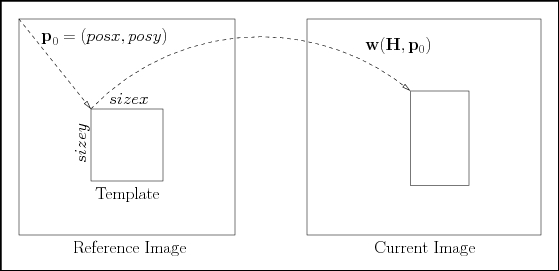
\includegraphics[width=1.0\textwidth]{tracking/figures/scale}
\caption{Translation and scaling of the reference template.}
\label{scale}
\end{center}
\end{figure}

In several applications, when tracking deformable objects it is better to fix the model to \lstinline$Rox_Tracking_Model_tu_tv_s$ or \lstinline$Rox_Tracking_Model_tu_tv_su_sv$.

% \subsubsection{Setting the parameters for tracking in the whole image or for target identification}
% \label{sss:tracking_params_ident}
% When the target make very large displacement in the image, it is sometimes necessary to search the target in the whole image. The same problem can arise when the target is lost, occluded or out of the image and the it comes back in the camera field of view. \rox{} allows the user to identify the target by choosing several identification methods using the following function:
% \begin{lstlisting}
% rox_tracking_params_set_ident(Rox_Tracking_Params P, Rox_Sint ident)
% \end{lstlisting}
% Setting ident to 0 will disable the research. The methods 1 and 2 are more robust but slower. The methods 2 and 4 are faster but the identification success rate is lower.

% The research time in the whole image may be a time consuming step. Thus it is possible to reduce the computation time by setting a parameters that tell to \rox{} to reduce the size of the image before the research. The use can use the following function:
% \begin{lstlisting}
% rox_tracking_params_set_ident_full_image(Rox_Tracking_Params P, Rox_Bool ident_full_image)
% \end{lstlisting}


\section{Tracking}
\label{sec:tracking}


\subsection{The Rox\_Tracking object}
\label{sse:tracking_object}

A \lstinline$Rox_Tracking$ object can be defined using the pointer to a \lstinline$Rox_Tracking_Structure$:
\begin{lstlisting}
typedef struct Rox_Tracking_Struct* Rox_Tracking;
\end{lstlisting}

\subsection{Creating/Deleting a Rox\_Tracking object}
\label{sss:track2d_initializing}

Functions are provided to allocate and deallocate a \lstinline$Rox_Tracking$ structure~:
\begin{lstlisting}
Rox_Tracking rox_tracking_new(Rox_Tracking_Params P, Rox_Camera C);
\end{lstlisting}
The \lstinline$rox_tracking_new$ function allocates memory for the structure of the track object, according to
the `P' parameters and returns a pointer on the newly created structure. \\

% \begin{lstlisting}
% Rox_Tracking rox_tracking_new_rect (
% 	Rox_Image 	I, 
% 	Rox_Window 	W,
% 	Rox_Uint 	miter, 
% 	Rox_Uint 	mprec, 
% 	Rox_Uint 	mpred);
% \end{lstlisting}
% The \lstinline$rox_tracking_new_rect$ function allocates memory for polygon and initialize it according to parameter `W' 
% and returns a pointer on the newly created structure. \\

% \begin{lstlisting}
% Rox_Tracking rox_tracking_new_poly (	
% 	Rox_Image 	I, 
% 	Rox_Sint 	*pts, 
% 	Rox_Sint 	nb_pts, 
% 	Rox_Uint 	miter, 
% 	Rox_Uint 	mprec, 
% 	Rox_Uint 	mpred);
% \end{lstlisting}

% The \lstinline$rox_tracking_new_rect$ function allocates memory for polygon and initialize it according to parameter `nb\_pts' 
% and returns a pointer on the newly created structure.

%%%%%%%%%%%%%%%%%%%%%%%%%% User: Odometry and Tracking %%%%%%%%%%%%%%%%%%%%%%%%%%%%%%%%%%%%
% \ifthenelse{\boolean{USER_TRACKING} \or \boolean{USER_ODOMETRY}}
% {
% The variables {\tt miter} and {\tt mprec} shall be initialized by the
% user. The variable {\tt miter} contains the maximum number of
% iterations for the minimization algorithm and the {\tt mprec} number
% corresponds to the precision of the tracking result. Both numbers
% should be always bigger than (or equal to) {\tt 1}. The user sets
% these numbers depending on the frame-rate of the acquisition of the
% images, on the power of the computer used and on the size of the
% template to track. For an acquisition frame-rate around 30 fps and a
% processor equivalent to Pentium IV 2GHz, setting {\tt miter = 10} and
% {\tt mprec = 3} gives good results when tracking a {\tt
%   (150}$\times${\tt 150)} template.
% The parameter  {\tt mpred} is a positive integer defining a search area around the template. 
% Setting the value of {\tt mpred} big allows handle important inter-frame displacements (the displacements of the target in two consecutive images can be big). 
% However, this slows down the visual tracking. A value of {\tt mpred} equal to {\tt 8} is a good compromise between speed and robustness. \\
% }
%%%%%%%%%%%%%%%%%%%%%%%%%% End of User: Odometry and Tracking %%%%%%%%%%%%%%%%%%%%%%%%%%%%%%%%%%%%
% \noindent These functions allocate memory for the \lstinline$Rox_Tracking$ structure and its field, 
% build image pyramid(s) from the reference patch / list of references patches and set
% the initial homography to the $3 \times 3$ identity matrix. If one does not want
% to build and use image pyramids, just set mprec to zero.\\

\begin{lstlisting}
Rox_Void rox_tracking_del(Rox_Tracking T);
\end{lstlisting}
The \lstinline$rox_tracking_del$ function deallocates memory for a \lstinline$Rox_Tracking$ structure. 
It is necessary to call this function when the structure is not used any more or before overwriting it. \\

The \lstinline$Rox_Tracking$ structure is opaque, i.e. its internal fields are hidden
and cannot be accessed directly by the user. A
consequence is that the user can only declare and manipulate pointer on this
structure, and never the structure itself, as the size of the structure 
is unknown to the user.\\

% In case of list of several patches, all of them shall be coplanar. Each can be
% generated using the `new' tool described above. The different patches are not
% tracked individually~: they are all unified in a unique system to solve. Thus,
% there is only one resulting homography, which correspond to the motion of the
% plane they belong to. \\

In order to track individually several patches, the user can declare and create
several \lstinline$Rox_Tracking$ structures and perform the algorithm on each of
them. The patches may also belong to different planes.\\

% \pagebreak %Specific

\subsection{The main functions related to the object Rox\_Tracking}
\label{sss:tracking_methods}

Once the \lstinline$Rox_Tracking$ is allocated and initialized, it is possible to:
\begin{itemize}
  \item Predict large motion
  \item Perform tracking pf planar objects
  \item Change tracking parameters
  \item Set the mask to track a generic template
  \item Measure the quality of the tracking
\end{itemize}


\subsubsection{Prediction}
\label{sse:prediction}

%\paragraph{Motivation}
%\label{par:prediction-motivation}

When a huge displacement occurs
between two frames of a sequence, due either to a fast motion or to a
low frame rate, the tracked object can get ``lost''.\\

In order to handle large displacement,
a phase of prediction can be introduced prior to the tracking
algorithm. It has to find the tracked object in a search window to
determine a translation applied to the current homography matrix and
then some iterations of the tracking algorithm can locally refine
the displacement.\\

The search window is set by the `mpred' parameter of the tracking
structure, which defines the number of pixels around the current
position of the tracked object.\\

As the prediction may be an expensive process, it is possible to skip it by
setting the `mpred' tracking parameter to zero.

\subsubsection{Perform tracking of planar objects}
\label{sss:tracking_perform}

To perform the tracking we call the \lstinline$rox_tracking_make$ function with the \lstinline$Rox_Tracking$ structure 
and the camera containing the image where to perform the tracking as parameters. This function shall be called for each image of the sequence. 

The resulting homography can be retrieved using the function:
\begin{lstlisting}
rox_tracking_get_matsl3_copy
\end{lstlisting}

which
returns a pointer on a $3 \times 3$ matrix. This homography can be used for example to draw a black box around the tracked
object in the image sequence, using the function:
\begin{lstlisting}
rox_image_draw_target_grays
\end{lstlisting}

\rox{} provides two functions that allow to access the reference and current template warped in the coordinate system 
of the reference template using the obtained homography:
\begin{description}
  \item \lstinline$rox_tracking_get_image_roi_ref$~: Returns the reference ROI.
  \item \lstinline$rox_tracking_get_image_roi_cur$~: Returns the current ROI warped in the coordinate system of the reference template using the obtained homography matrix.
\end{description}

\subsubsection{Changing the Tracking Parameters during runtime}
\label{sss:track2D_setparam}

The tracking algorithm has four parameters set at the
\lstinline$Rox_Tracking$ structure initialization~: `miter', `mprec',
`msamp' and `mpred'. However, it is not mandatory to use the same
parameters during the whole sequence. For example, a part of the
sequence may need a prediction phase and few iterations because of a
known high translation, but we would rather use more iterations
without prediction for the rest of the sequence.\\

The list of functions that allow the user to set tracking parameters
are given in the Programmer Manual.  They can change at any
moment. Setting a parameter with a strictly negative value (typically
-1) will leave it unchanged.
%The only thing you cannot change after the initialization
%is whether to build and use image pyramids~: setting a null value for
%`mprec' after initialization will not delete the pyramids, nor a
%positive value will create it.
\\

%Warning ! If a null value is set for `miter' and / or `mprec', no iteration at
%all of the ESM algorithm will be performed ! If `mpred' is not null, a tracking
%only based on the prediction will be performed, else there will be no tracking
%at all.

\subsubsection{Setting the mask to track a generic template}
\label{sss:track2D_generic_template}

\rox{} allows the user to perform the visual tracking of non-rectangular templates in the reference image. 
The function \lstinline$rox_tracking_set_imask$ shall be used for such templates.\\
Further information about mask can be found in section \ref{sec:imask}. Tracking can then be performed with \lstinline$rox_tracking_make$ function.

\subsubsection{Measuring the quality of the visual tracking}
\label{sss:track2D_measure_quality}

In order to obtain the quality of the tracking result, the function
\lstinline$rox_tracking_get_score$ uses the Zero-mean Normalized
Cross-Correlation (ZNCC) between the reference template and the
current image warped in the coordinate system of the reference
template.\\

If we denote by $I_r$ and $I_c$ the vectors containing the intensity values of the reference template and of the current warped image and
 by $\overline{I_r}$ and $\overline{I_c}$ the means of the vectors $I_r$ and $I_c$, the ZNCC can be written as follows:
\begin{displaymath}
ZNCC(I_r, I_c) = \frac{(I_r - \overline{I_r}) \cdot (I_c - \overline{I_c})}
{||I_r - \overline{I_r}|| \times ||I_c - \overline{I_c}||}
\end{displaymath}
The value of the ZNCC is between {\tt -1.0} and {\tt 1.0}. When the reference template and the current template are identical, the ZNCC is equal to {\tt 1.0}. 
When the reference template and the current template are completely different, the ZNCC is close to {\tt -1.0}.
Therefore, the ZNCC is a very good measure that provides the quality of the visual tracking. 
When the reference template is tracked correctly, the returned value of the ZNCC is close to {\tt 1.0} (or bigger than {\tt 0.75} for example).

The score s used by \rox{} is normalized between 0 and 1 as follows:
\[
s = (ZNCC+1.0)/2.0
\]

See the example ``rox\_example\_tracking.tex'' for an example of use.

%\input{tracking/rox_example_tracking}

%\input{tracking/track3D}

\newpage
\chapter{Odometry Module}
\label{cha:vodom}
Visual odometry is the process of determining the position and
orientation (the pose) of a camera relative to a given target by
analyzing a sequence of images. Contrarily to object tracking in
image coordinates, visual odometry needs calibrated cameras. It 
implies the knowledge of camera intrinsic parameters. Consequently, 
the \lstinline$Rox_Camera$ object shall be fed with the correct 
camera  intrinsic parameters. Incorrect camera intrinsic parameters
will produce an incorrect localization.

The localization of the camera in the environment can be useful in several applications such as robotics, augmented reality, and many others.\\

The Odometry module contains the following sub-modules:

\begin{description}
% \item[Odometry Parameters]~: module with structures and methods for handling the tracking parameters
  \item[Odometry Single Plane]~: module with structures and methods for camera localization relative to a single plane
  \item[Odometry Multi Planes]~: module with structures and methods for camera localization relative to a multi planes
  \item[Odometry Inertial Observer]~: module with structures and methods for camera localization with inertial observer
\end{description}

\section{Visual odometry observing a single plane}
\label{sec:vodm_single_plane}

\subsection{Odometry parameters}
\label{sse:odometry_single_plane_params}

\subsubsection{The {\tt Rox\_Odometry\_Params} object}
\label{sss:odometry_single_plane_params_object}

A \lstinline$Rox_Odometry_Single_Plane_Params$ object can be defined using the pointer to a \lstinline$Rox_Tracking_Params_Structure$:
\begin{lstlisting}
typedef struct Rox_Tracking_Params_Struct* Rox_Odometry_Single_Plane_Params;
\end{lstlisting}
The structure is opaque to the users.

\subsubsection{Creating/Deleting a {\tt Rox\_Odometry\_Params}}
\label{sss:odometry_single_plane_params_newdel}

Functions are provided to allocate and deallocate a \lstinline$Rox_Odometry_Single_Plane_Params$ object~:

\begin{lstlisting}
Rox_Error rox_odometry_single_plane_params_new (Rox_Odometry_Single_Plane_Params *params);
\end{lstlisting}
The \lstinline$rox_odometry_single_plane_params_new$ function allocates memory for the odometry object and returns a pointer on the newly created object.

\begin{lstlisting}
Rox_Error rox_odometry_single_plane_params_del (Rox_Odometry_Single_Plane_Params *params);
\end{lstlisting}
The function deallocates memory for a \lstinline$Rox_Odometry_Single_Plane_Params$ object. It is necessary to call this function when the object is not used anymore. \\

\subsubsection{Main functions related to {\tt Rox\_Odometry\_Params}}
\label{sss:odometry_single_plane_params_methods}

% \paragraph{Localization relative to objects with known size}
% \label{par:odometry_model}
% ~\\~\\
The camera localization is done relative to a known object. It is
assumed that a rectangular planar object with size (sizx, sizy) is
observed. In this case it is possible to know the pose of the camera
relative to the planar object (the object frame is centered on the
rectangular object, see figure~\ref{model_size}) and also the
displacement of the camera between two images.

\begin{figure}[htbp] 
\begin{center}
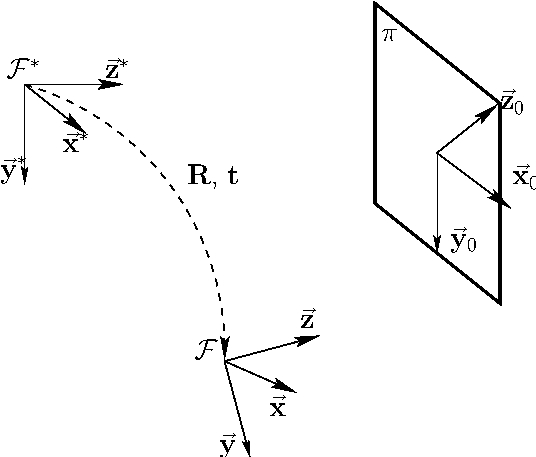
\includegraphics[width=0.75\textwidth]{odometry/figures/model_size}
\caption{Localization relative to a planar object with known size.}
\label{model_size}
\end{center}
\end{figure}

% \paragraph{Localization relative to objects with known normal}
% \label{par:odometry_scale}
% ~\\~\\
% If the camera localization is done relative to a known object the user shall set the scaled normal of the plane using the following function:

% \begin{lstlisting}
% Rox_Void rox_odometry_single_plane_params_set_model_normal(Rox_Odometry_Single_Plane_Params P, Rox_Vector nd)
% \end{lstlisting}

% \begin{figure}[htbp] 
% \begin{center}
% 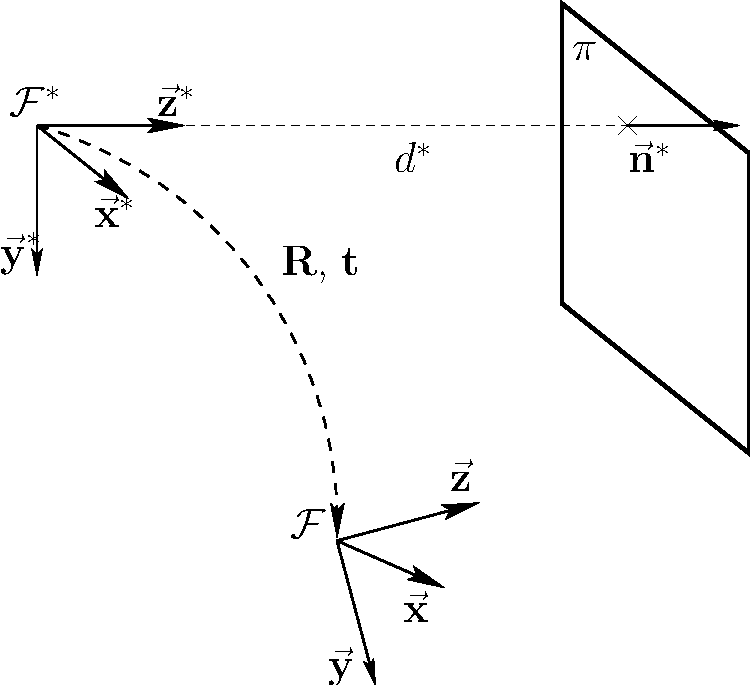
\includegraphics[width=0.5\textwidth]{odometry/figures/model_norm}
% \caption{Localization relative to a planar object with unknown size.}
% \label{model_norm}
% \end{center}
% \end{figure}



\subsection{Visual odometry Single Plane}
\label{sse:odometry_single_plane}

\subsubsection{The {\tt Rox\_Odometry\_Single\_Plane} object}
\label{sss:odometry_single_plane_object}

A \lstinline$Rox_Odometry_Single_Plane$ is a pointer to the opaque structure \lstinline$Rox_Odometry_Single_Plane_Structure$:
\begin{lstlisting}
typedef struct Rox_Odometry_Single_Plane_Struct *Rox_Odometry_Single_Plane;
\end{lstlisting}

\subsubsection{Creating/Deleting a {\tt Rox\_Odometry\_Single\_Plane}}
\label{sss:odometry_single_plane_newdel}
Functions are provided to allocate and deallocate a \lstinline$Rox_Odometry_Single_Plane$ object~:

\begin{lstlisting}
Rox_Error rox_odometry_single_plane_new (Rox_Odometry_Single_Plane *odometry, Rox_Odometry_Single_Plane_Params params, Rox_Model_Single_Plane model);
\end{lstlisting}
The function allocates memory for the odometry object, according to
the 'model' and `params' parameters and returns a pointer on the newly created object.

\begin{lstlisting}
Rox_Error rox_odometry_single_plane_del (Rox_Odometry_Single_Plane *odometry);
\end{lstlisting}
The function deallocates memory for a \lstinline$Rox_Odometry_Single_Plane$ object. 
It is necessary to call this function when the object is not used anymore. \\

\subsubsection{Main functions related to {\tt Rox\_Odometry\_Single\_Plane}}
\label{sss:odometry_single_plane_methods}
The main functions to manipulate a \lstinline$Rox_Odometry$ object are~:
\begin{description}
  \item[rox\_odometry\_single\_plane\_make]: Performs the visual odometry when the
  displacement of the target is not too large~;
  \item[rox\_odometry\_single\_plane\_get\_pose]: Returns the pose matrix~;
  \item[rox\_odometry\_single\_plane\_set\_pose]: Set the pose matrix~;
  \item[rox\_odometry\_single\_plane\_get\_score]: Returns the quality score of visual odometry~;
\end{description}

Please refer to the Programmer Manual for further information about visual odometry functions, 

\subsubsection{Target identification}
\label{sss:odometry_single_plane_dent}
~\\~\\
When the displacement of the target is very large in the image, it is sometimes necessary to search the target in the whole image. The same problem can arise when the target is lost, occluded or out of the image and comes back in the camera field of view. \rox{} allows the user to identify the target by choosing several identification methods. The methods are detailed in section~\ref{sec:ident}. See the example ``rox\_example\_odometry\_single\_plane.c'' for odometry with identification using a textured image and ``rox\_example\_odometry\_single\_plane\_database.c'' for odometry with identification using a database of textured images.

If the user needs a very robust identification we recommend to use a
photoframe around the target. Section \ref{sse:ident_photoframe}
describes how to build photoframes and use them for target
identification.  See the example ``rox\_example\_odometry\_single\_plane\_photoframe.c'' for an
example of use with the odometry.

% \input{odometry/rox_example_odometry.tex}
% \input{odometry/rox_example_odometry_photoframe.tex}


\section{Visual odometry observing multi planes}
\label{sec:vodm_multi_plane}

%\input{odometry/odometry_m3d_params.tex}

\subsection{Visual Odometry Multi Plane}
\label{sse:odometry_multi_plane}

The odometry module enables tracking of a textured convex polyhedron of $n$ faces whose real
dimensions are known. The estimation of the camera pose is obtained whatever the part of the object the 
camera is looking at. The object is considered as a whole and the module uses all visible information 
to get a precise and stable localization of the object. The simplest example of a convex polyhedron 
is a cube (6 faces). The object to track using this module shall be textured on all the faces. Constraints
related to texture are similar to those of 2D planar odometry. 

\subsubsection{The {\tt Rox\_Odometry\_Multi\_Plane} object}
\label{sss:odometry_multi_plane_object}

A \lstinline$Rox_Odometry_Multi_Plane$ object is a pointer to the \lstinline$Rox_Odometry_Multi_Plane_Struct$ structure:
\begin{lstlisting}
typedef struct Rox_Odometry_Multi_Plane_Struct* Rox_Odometry_Multi_Plane;
\end{lstlisting}
The structure is opaque to the users.

\subsubsection{Creating/Deleting a {\tt Rox\_Odometry\_Multi\_Plane}}
\label{sss:odometry_multi_plane_newdel}
Functions are provided to allocate and deallocate a \lstinline$Rox_Odometry_Multi_Plane$ object~:

\begin{lstlisting}
Rox_Odometry_Multi_Plane rox_odometry_multi_plane_new(Rox_Odometry_Multi_Plane_Params params, Rox_Model_Multi_plane model);
\end{lstlisting}
The function allocates memory for the odometry object, according to the {\tt model} and {\tt params} parameters and returns a pointer on the newly created object.

A 3D object model shall be passed to the odometry module for an appropriate odometry process (see section~\ref{sec:model_multi_plane}). 
The precision of the 3D vertices passed as input is the key to the accuracy of the odometry results. 3D vertices are used 
to simulate the object image projection. If the vertices are not well defined, the alignment of the real object and the virtual 
object is not possible. Scale of the vertices is not important for the visual odometry. However the output pose varies with 
the input scale.

Carefully choosing textures is very important for a robust odometry. The picture captured for each quadrilateral shall be as much 
parallel as possible relative to the face. Blur, noise and other lighting artefacts shall be avoided. Textures shall be as big as 
possible (e.g. a 512{*}512 texture per quadrilateral). If possible, use the same device for capturing the texture and for the 
odometry process, in order to minimize differences between images.

\begin{lstlisting}
Rox_Void rox_odometry_multi_plane_del(Rox_Odometry_Multi_Plane odometry);
\end{lstlisting}
The \lstinline$rox_odometry_multi_plane_del$ function deallocates memory for a \lstinline$Rox_Odometry_Multi_Plane$ object. It is necessary to call this function when the object is not used anymore. \\

\subsubsection{Main functions related to {\tt Rox\_Odometry\_Multi\_Plane}}
\label{sss:odometry_multi_plane_methods}

The main functions to manipulate a \lstinline$Rox_Odometry_Multi_Plane$ object are~:
\begin{description}
  \item[rox\_odometry\_multi\_plane\_make]: Performs the visual odometry and update the camera pose~;
  \item[rox\_odometry\_multi\_plane\_get\_pose]: Returns the pose matrix~;
  \item[rox\_odometry\_multi\_plane\_set\_pose]: Set the pose matrix~;
  % \item[rox\_odometry\_get\_score]: Returns the quality score of visual odometry~;
\end{description}

Please refer to the Programmer Manual for further information about visual odometry functions.
See the example ``rox\_example\_odometry\_multi\_plane.c'' for an example of use.


\section{Visual odometry with an inertial observer}

\subsection{Visual and Inertial Odometry}
\label{sse:odometry_visual_inertial}

When the displacement between two successive images is too large, the visual odometry may fail. Consequently, it is necessary to identify the target to get the camera pose relative to the known model. Using an inertial sensor allows us to get a high rate prediction of the target position in the image even if the displacement is very important. The visual odometry may be successful as long as the inertial prediction is precise enough. As the inertial prediction does not depend on the actual scene viewed by the camera, it is possible to predict the target position even if it is out of the camera field of view. Consequently, when the target reappears in the camera field of view, no identification method will be necessary to make visual odometry if the inertial prediction is close enough from the real target position. \\
Note that to make an efficient visual - inertial odometry, the calibration pose between the two sensors shall be known by the user and the target frame shall coincide with the local tangent plane used as reference for the inertial measures.    

\subsubsection{Main functions related to {\tt Rox\_Odometry\_Visual\_Inertial}}
\label{sss:odometry_visual_inertial_methods}

The main functions to manipulate visual - inertial odometry are~:
\begin{description}
  \item[rox\_odometry\_visual\_inertial\_init\_async\_observer]: Performs the detection of the given target and initializes the inertial observer using the odometry results. This function initializes an asynchronous observer implying that visual and inertial data have to be precisely dated. The dating shall be expressed in seconds and have the same time reference for both inertial and visual data (i.e using the UTC time)~;
  \item[rox\_odometry\_visual\_inertial\_init\_sync\_observer]: Performs the detection of the given target and initializes the inertial observer using the odometry results. This function initializes a synchronous observer~;
  \item[rox\_odometry\_visual\_inertial\_make]: Makes the visual - inertial odometry. Note that the inertial observer can be reinitialized by a visual detection method if the target has been lost during 10 successive images~;
  \item[rox\_odometry\_visual\_inertial\_get\_matsl3\_prediction\_copy]: Gets a copy of the initialization homography~;
\end{description}

If you need further information about visual and inertial odometry functions, please refer to the Programmer Manual.
See the example ``rox\_example\_odometry\_visual\_inertial.tex'' for an
example of use.

% \input{odometry/rox_example_odometry_visual_inertial.tex}



%\appendix
%\include{appendix/coding}
% \include{appendix/compatibility}
% \include{examp/sampleprogram}
% \include{appendix/algorithm}
% \chapter{Model Module}
\label{cha:model}
The model module contains structures and methods for model manipulation.\\

The model module contains the following sub-modules~:

\begin{description}
  \item[Model Single Plane]~: Module with structures and methods for single plane models definition and use~;
  \item[Model Multi Plane]~: Module with structures and methods for multi plane models definition and use~;
\end{description}

\section{Model Single Plane}
\label{sec:model_single_plane}

\subsection{The {\tt Rox\_Model\_Single\_Plane} object}
\label{sse:model_single_plane_typedef}
A \lstinline$Rox_Model_Single_Plane$ object can be declared using the pointer to a \lstinline$Rox_Model_Single_Plane_Struct$: 

\begin{lstlisting}
typedef struct Rox_Model_Single_Plane_Struct* Rox_Model_Single_Plane;
\end{lstlisting}

The structure is opaque to the user and can only be accessed through constructors, destructors and methods described in the following sections.

\subsection{Creating/Deleting a {\tt Rox\_Model\_Single\_Plane}}
\label{sse:model_single_plane_newdel}

Functions are provided to allocate, initialize and deallocate an \lstinline$Rox_Model_Single_Plane$ object~:
\begin{lstlisting}
Rox_Error rox_model_single_plane_new(Rox_Model_Single_Plane * model_single_plane, Rox_Image image, Rox_Real sizex, Rox_Real sizey);
\end{lstlisting}
The \lstinline$rox_model_single_plane_new$ function allocates memory for data. \\ 

\begin{lstlisting}
Rox_Error rox_model_single_plane_del(Rox_Model_Single_Plane * model_single_plane);
\end{lstlisting}
The \lstinline$rox_model_single_plane_del$ function deallocates memory for an \lstinline$Rox_Model_Single_Plane$ structure. It is necessary to call this function when the
structure is not used any more or before overwriting it.

\subsection{Main functions related to {\tt Rox\_Model\_Single\_Plane}}
\label{sse:model_single_plane_functs}
The texture (i.e. an image) associated to the planar model can be set using the following function:
\begin{lstlisting}
Rox_Error rox_model_single_plane_set_template(Rox_Model_Single_Plane model, Rox_Image image, Rox_Real sizex, Rox_Real sizey); 
\end{lstlisting}
The real size of the planar target must be given.

\section{Model Multi Plane}
\label{sec:model_multi_plane}
The present version of \rox{} allows the user to define simple 3D objects only.
Currently, the 3D object is described as a set of 3D quadrilaterals (e.g. : the 6 
faces of a cube or parts of the faces). Each quadrilateral is defined by an image 
texture and four 3D points associated to each corner of the texture (order : Top left -> Top
right -> Bottom right -> Bottom left). The 3D vertices of all faces shall be defined 
in a common reference frame $\mathcal{F}_{r}$. Be sure to define your 3D coordinates 
as precisely as possible. It is up to the user to choose the adequate $\mathcal{F}_{r}$ for your vertices.
The default pose estimated by the odometry is the 3D transformation 
(rotation and translation) from this reference frame to the camera frame. 

\subsection{The {\tt Rox\_Model\_Multi\_Plane} object}
\label{sse:model_multi_plane_struct}
A model 3D object is a pointer to the opaque structure \lstinline$Rox_Model_Multi\_Plane_Struct$: 

\begin{lstlisting}
typedef struct Rox_Model_Multi\_Plane_Struct* Rox_Model_Multi\_Plane;
\end{lstlisting}

The structure is opaque to the user and can only be accessed through constructors, destructors and methods described in the following sections.

\subsection{Creating/Deleting a {\tt Rox\_Model\_Multi\_Plane}}
\label{sse:model_multi_plane_newdel}

Functions are provided to allocate, initialize and deallocate an \lstinline$Rox_Model_Multi\_Plane$ object~:
\begin{lstlisting}
Rox_Error rox_model_multi_plane_new(Rox_Model_Multi\_Plane * model_multi_plane);
\end{lstlisting}
The \lstinline$rox_model_multi_plane_new$ function allocates memory for data. \\ 

\begin{lstlisting}
Rox_Error rox_model_multi_plane_del(Rox_Model_Multi\_Plane * model_multi_plane);
\end{lstlisting}
The \lstinline$rox_model_multi_plane_del$ function deallocates memory for an \lstinline$Rox_Model_Multi_Plane$ structure. It is necessary to call this function when the
structure is not used any more or before overwriting it.

\subsection{Main functions related to {\tt Rox\_Model\_Multi\_Plane}}
\label{sse:model_multi_plane_functs}

The main function related to the \lstinline$Rox_Model_Multi_Plane$ is the function that allows to define an additional textured quadrilateral belonging to the 3D object:
\begin{lstlisting}
Rox_Error rox_model_multi_plane_append_plane(Rox_Model_Multi_Plane model, Rox_Image image, Rox_Real vertices[4])
\end{lstlisting}


% \include{appendix/performance}
% \bibliographystyle{plain}

%\addcontentsline{toc}{section}{References}
%\bibliography{biblio/references}
\printindex

\end{document}
